% Options for packages loaded elsewhere
\PassOptionsToPackage{unicode}{hyperref}
\PassOptionsToPackage{hyphens}{url}
\PassOptionsToPackage{dvipsnames,svgnames,x11names}{xcolor}
%
\documentclass[
]{article}

\usepackage{amsmath,amssymb}
\usepackage{iftex}
\ifPDFTeX
  \usepackage[T1]{fontenc}
  \usepackage[utf8]{inputenc}
  \usepackage{textcomp} % provide euro and other symbols
\else % if luatex or xetex
  \usepackage{unicode-math}
  \defaultfontfeatures{Scale=MatchLowercase}
  \defaultfontfeatures[\rmfamily]{Ligatures=TeX,Scale=1}
\fi
\usepackage{lmodern}
\ifPDFTeX\else  
    % xetex/luatex font selection
\fi
% Use upquote if available, for straight quotes in verbatim environments
\IfFileExists{upquote.sty}{\usepackage{upquote}}{}
\IfFileExists{microtype.sty}{% use microtype if available
  \usepackage[]{microtype}
  \UseMicrotypeSet[protrusion]{basicmath} % disable protrusion for tt fonts
}{}
\makeatletter
\@ifundefined{KOMAClassName}{% if non-KOMA class
  \IfFileExists{parskip.sty}{%
    \usepackage{parskip}
  }{% else
    \setlength{\parindent}{0pt}
    \setlength{\parskip}{6pt plus 2pt minus 1pt}}
}{% if KOMA class
  \KOMAoptions{parskip=half}}
\makeatother
\usepackage{xcolor}
\setlength{\emergencystretch}{3em} % prevent overfull lines
\setcounter{secnumdepth}{5}
% Make \paragraph and \subparagraph free-standing
\ifx\paragraph\undefined\else
  \let\oldparagraph\paragraph
  \renewcommand{\paragraph}[1]{\oldparagraph{#1}\mbox{}}
\fi
\ifx\subparagraph\undefined\else
  \let\oldsubparagraph\subparagraph
  \renewcommand{\subparagraph}[1]{\oldsubparagraph{#1}\mbox{}}
\fi


\providecommand{\tightlist}{%
  \setlength{\itemsep}{0pt}\setlength{\parskip}{0pt}}\usepackage{longtable,booktabs,array}
\usepackage{calc} % for calculating minipage widths
% Correct order of tables after \paragraph or \subparagraph
\usepackage{etoolbox}
\makeatletter
\patchcmd\longtable{\par}{\if@noskipsec\mbox{}\fi\par}{}{}
\makeatother
% Allow footnotes in longtable head/foot
\IfFileExists{footnotehyper.sty}{\usepackage{footnotehyper}}{\usepackage{footnote}}
\makesavenoteenv{longtable}
\usepackage{graphicx}
\makeatletter
\def\maxwidth{\ifdim\Gin@nat@width>\linewidth\linewidth\else\Gin@nat@width\fi}
\def\maxheight{\ifdim\Gin@nat@height>\textheight\textheight\else\Gin@nat@height\fi}
\makeatother
% Scale images if necessary, so that they will not overflow the page
% margins by default, and it is still possible to overwrite the defaults
% using explicit options in \includegraphics[width, height, ...]{}
\setkeys{Gin}{width=\maxwidth,height=\maxheight,keepaspectratio}
% Set default figure placement to htbp
\makeatletter
\def\fps@figure{htbp}
\makeatother

\usepackage[noblocks]{authblk}
\renewcommand*{\Authsep}{, }
\renewcommand*{\Authand}{, }
\renewcommand*{\Authands}{, }
\renewcommand\Affilfont{\small}
\setlength{\tabcolsep}{3pt}
\usepackage{longtable}
\usepackage{array}
\makeatletter
\makeatother
\makeatletter
\makeatother
\makeatletter
\@ifpackageloaded{caption}{}{\usepackage{caption}}
\AtBeginDocument{%
\ifdefined\contentsname
  \renewcommand*\contentsname{Table of contents}
\else
  \newcommand\contentsname{Table of contents}
\fi
\ifdefined\listfigurename
  \renewcommand*\listfigurename{List of Figures}
\else
  \newcommand\listfigurename{List of Figures}
\fi
\ifdefined\listtablename
  \renewcommand*\listtablename{List of Tables}
\else
  \newcommand\listtablename{List of Tables}
\fi
\ifdefined\figurename
  \renewcommand*\figurename{Figure}
\else
  \newcommand\figurename{Figure}
\fi
\ifdefined\tablename
  \renewcommand*\tablename{Table}
\else
  \newcommand\tablename{Table}
\fi
}
\@ifpackageloaded{float}{}{\usepackage{float}}
\floatstyle{ruled}
\@ifundefined{c@chapter}{\newfloat{codelisting}{h}{lop}}{\newfloat{codelisting}{h}{lop}[chapter]}
\floatname{codelisting}{Listing}
\newcommand*\listoflistings{\listof{codelisting}{List of Listings}}
\makeatother
\makeatletter
\@ifpackageloaded{caption}{}{\usepackage{caption}}
\@ifpackageloaded{subcaption}{}{\usepackage{subcaption}}
\makeatother
\makeatletter
\@ifpackageloaded{tcolorbox}{}{\usepackage[skins,breakable]{tcolorbox}}
\makeatother
\makeatletter
\@ifundefined{shadecolor}{\definecolor{shadecolor}{rgb}{.97, .97, .97}}
\makeatother
\makeatletter
\makeatother
\makeatletter
\makeatother
\ifLuaTeX
  \usepackage{selnolig}  % disable illegal ligatures
\fi
\IfFileExists{bookmark.sty}{\usepackage{bookmark}}{\usepackage{hyperref}}
\IfFileExists{xurl.sty}{\usepackage{xurl}}{} % add URL line breaks if available
\urlstyle{same} % disable monospaced font for URLs
\hypersetup{
  pdfauthor={Paweł Wiczling*},
  colorlinks=true,
  linkcolor={blue},
  filecolor={Maroon},
  citecolor={Blue},
  urlcolor={Blue},
  pdfcreator={LaTeX via pandoc}}

\title{Supporting Information for:\\
An Interpretable Multilevel Model of Isocratic Retention Explaining
Between-Analyte and Between-Column Variability}


  \author{Paweł Wiczling*}
            \affil{%
                  Department of Biopharmaceutics and Pharmacodynamics,
                  Medical University of Gdańsk, Gen.~J. Hallera 107,
                  80-416 Gdańsk, Poland
              }
      
\date{2026-07-27}
\begin{document}
\maketitle
\ifdefined\Shaded\renewenvironment{Shaded}{\begin{tcolorbox}[frame hidden, boxrule=0pt, borderline west={3pt}{0pt}{shadecolor}, sharp corners, breakable, enhanced, interior hidden]}{\end{tcolorbox}}\fi

\renewcommand*\contentsname{Table of contents}
{
\hypersetup{linkcolor=}
\setcounter{tocdepth}{3}
\tableofcontents
}
\newpage{}

\hypertarget{table-s1.-summary-of-the-mcmc-simulations-of-the-marginal-posterior-distributions-of-population-level-model-parameters.}{%
\section{Table S1. Summary of the MCMC simulations of the marginal
posterior distributions of population-level model
parameters.}\label{table-s1.-summary-of-the-mcmc-simulations-of-the-marginal-posterior-distributions-of-population-level-model-parameters.}}

Summary of posterior parameter estimates. The table reports posterior
summaries for each parameter, including measures of central tendency
(mean, median), uncertainty (standard deviation, median absolute
deviation, and 5th/95th percentiles), and MCMC diagnostic statistics
(rhat, bulk effective sample size, and tail effective sample size).

\begingroup\fontsize{7}{9}\selectfont

\begin{longtable*}[t]{l|r|r|r|r|r|r|r|r|r}
\hline
variable & mean & median & sd & mad & q5 & q95 & rhat & ess\_bulk & ess\_tail\\
\hline
\endfirsthead
\multicolumn{10}{@{}l}{\textit{(continued)}}\\
\hline
variable & mean & median & sd & mad & q5 & q95 & rhat & ess\_bulk & ess\_tail\\
\hline
\endhead
logkw\_hat & 3.1600 & 3.160 & 0.149 & 0.142 & 2.91000 & 3.4000 & 1.01 & 465 & 1200\\
\hline
S1\_hat & 3.9500 & 3.950 & 0.124 & 0.119 & 3.74000 & 4.1500 & 1.01 & 422 & 841\\
\hline
logS2\_hat & 0.3230 & 0.323 & 0.032 & 0.033 & 0.27000 & 0.3760 & 1.00 & 1050 & 2210\\
\hline
fid\_hat & 0.0121 & 0.015 & 0.009 & 0.007 & -0.00670 & 0.0212 & 1.00 & 1640 & 2490\\
\hline
alpha\_hat & 4.7300 & 4.730 & 0.062 & 0.063 & 4.63000 & 4.8400 & 1.00 & 3130 & 3520\\
\hline
dlogkw\_hat & -2.3800 & -2.380 & 0.083 & 0.081 & -2.51000 & -2.2500 & 1.00 & 2050 & 2610\\
\hline
dS1\_hat & 2.1600 & 2.160 & 0.251 & 0.245 & 1.75000 & 2.5700 & 1.00 & 3710 & 2780\\
\hline
dlogS2\_hat & -0.8620 & -0.862 & 0.054 & 0.053 & -0.95200 & -0.7720 & 1.00 & 1850 & 2760\\
\hline
gamma\_hat & 3.0600 & 3.090 & 0.412 & 0.416 & 2.36000 & 3.7100 & 1.00 & 2730 & 2820\\
\hline
beta\_a\_hat[1] & 0.8310 & 0.831 & 0.055 & 0.054 & 0.74000 & 0.9220 & 1.01 & 468 & 697\\
\hline
beta\_a\_hat[2] & 0.7400 & 0.740 & 0.054 & 0.053 & 0.65200 & 0.8280 & 1.01 & 554 & 739\\
\hline
beta\_c\_hat[1] & 0.7360 & 0.737 & 0.221 & 0.211 & 0.37000 & 1.1000 & 1.00 & 4890 & 2820\\
\hline
beta\_c\_hat[2] & 0.5430 & 0.547 & 0.185 & 0.184 & 0.24000 & 0.8510 & 1.00 & 3930 & 2780\\
\hline
beta\_c\_hat[3] & 0.2810 & 0.277 & 0.095 & 0.091 & 0.12800 & 0.4420 & 1.00 & 2640 & 2480\\
\hline
omega\_a[1] & 0.9920 & 0.988 & 0.071 & 0.072 & 0.88300 & 1.1100 & 1.01 & 698 & 1340\\
\hline
omega\_a[2] & 0.9160 & 0.914 & 0.069 & 0.069 & 0.80700 & 1.0300 & 1.01 & 709 & 1680\\
\hline
omega\_a[3] & 0.3450 & 0.344 & 0.025 & 0.024 & 0.30600 & 0.3880 & 1.01 & 723 & 1390\\
\hline
omega\_c[1] & 0.4260 & 0.415 & 0.088 & 0.081 & 0.30700 & 0.5870 & 1.00 & 2540 & 2550\\
\hline
omega\_c[2] & 0.3010 & 0.293 & 0.061 & 0.057 & 0.21700 & 0.4140 & 1.00 & 2380 & 2820\\
\hline
omega\_c[3] & 0.1010 & 0.098 & 0.021 & 0.019 & 0.07200 & 0.1380 & 1.00 & 2690 & 3030\\
\hline
omega\_c[4] & 1.2600 & 1.240 & 0.272 & 0.274 & 0.85300 & 1.7400 & 1.00 & 3520 & 3080\\
\hline
omega\_c[5] & 0.0119 & 0.009 & 0.008 & 0.006 & 0.00371 & 0.0284 & 1.00 & 1950 & 3040\\
\hline
omega\_c[6] & 0.2110 & 0.207 & 0.039 & 0.037 & 0.15300 & 0.2800 & 1.00 & 3160 & 2750\\
\hline
omega\_c[7] & 0.4660 & 0.465 & 0.069 & 0.069 & 0.35300 & 0.5820 & 1.00 & 3650 & 2300\\
\hline
omega\_c[8] & 0.1620 & 0.158 & 0.033 & 0.032 & 0.11600 & 0.2210 & 1.00 & 3870 & 3240\\
\hline
m\_logomega\_d[1] & -1.7900 & -1.790 & 0.199 & 0.190 & -2.10000 & -1.4400 & 1.01 & 1390 & 1650\\
\hline
m\_logomega\_d[2] & -2.0100 & -2.010 & 0.184 & 0.178 & -2.30000 & -1.7000 & 1.00 & 2230 & 2270\\
\hline
m\_logomega\_d[3] & -2.7100 & -2.730 & 0.400 & 0.384 & -3.34000 & -2.0300 & 1.00 & 2060 & 2700\\
\hline
sd\_logomega\_d[1] & 0.7130 & 0.692 & 0.143 & 0.132 & 0.52200 & 0.9730 & 1.00 & 1990 & 2720\\
\hline
sd\_logomega\_d[2] & 0.6350 & 0.614 & 0.131 & 0.119 & 0.45700 & 0.8760 & 1.00 & 2930 & 2670\\
\hline
sd\_logomega\_d[3] & 1.4400 & 1.400 & 0.306 & 0.282 & 1.02000 & 1.9900 & 1.00 & 1720 & 2660\\
\hline
rho\_a[1,1] & 1.0000 & 1.000 & 0.000 & 0.000 & 1.00000 & 1.0000 & NA & NA & NA\\
\hline
rho\_a[2,1] & 0.9380 & 0.940 & 0.014 & 0.013 & 0.91200 & 0.9580 & 1.01 & 885 & 1800\\
\hline
rho\_a[3,1] & 0.4450 & 0.450 & 0.077 & 0.078 & 0.30900 & 0.5630 & 1.01 & 798 & 1290\\
\hline
rho\_a[1,2] & 0.9380 & 0.940 & 0.014 & 0.013 & 0.91200 & 0.9580 & 1.01 & 885 & 1800\\
\hline
rho\_a[2,2] & 1.0000 & 1.000 & 0.000 & 0.000 & 1.00000 & 1.0000 & NA & NA & NA\\
\hline
rho\_a[3,2] & 0.3510 & 0.355 & 0.084 & 0.085 & 0.20500 & 0.4840 & 1.01 & 646 & 1460\\
\hline
rho\_a[1,3] & 0.4450 & 0.450 & 0.077 & 0.078 & 0.30900 & 0.5630 & 1.01 & 798 & 1290\\
\hline
rho\_a[2,3] & 0.3510 & 0.355 & 0.084 & 0.085 & 0.20500 & 0.4840 & 1.01 & 646 & 1460\\
\hline
rho\_a[3,3] & 1.0000 & 1.000 & 0.000 & 0.000 & 1.00000 & 1.0000 & NA & NA & NA\\
\hline
rho\_c[1,1] & 1.0000 & 1.000 & 0.000 & 0.000 & 1.00000 & 1.0000 & NA & NA & NA\\
\hline
rho\_c[2,1] & 0.8290 & 0.847 & 0.094 & 0.087 & 0.65300 & 0.9460 & 1.00 & 2750 & 2550\\
\hline
rho\_c[3,1] & 0.7090 & 0.727 & 0.123 & 0.122 & 0.47700 & 0.8820 & 1.00 & 3610 & 2760\\
\hline
rho\_c[1,2] & 0.8290 & 0.847 & 0.094 & 0.087 & 0.65300 & 0.9460 & 1.00 & 2750 & 2550\\
\hline
rho\_c[2,2] & 1.0000 & 1.000 & 0.000 & 0.000 & 1.00000 & 1.0000 & NA & NA & NA\\
\hline
rho\_c[3,2] & 0.7440 & 0.763 & 0.116 & 0.112 & 0.53100 & 0.8990 & 1.00 & 3100 & 2550\\
\hline
rho\_c[1,3] & 0.7090 & 0.727 & 0.123 & 0.122 & 0.47700 & 0.8820 & 1.00 & 3610 & 2760\\
\hline
rho\_c[2,3] & 0.7440 & 0.763 & 0.116 & 0.112 & 0.53100 & 0.8990 & 1.00 & 3100 & 2550\\
\hline
rho\_c[3,3] & 1.0000 & 1.000 & 0.000 & 0.000 & 1.00000 & 1.0000 & NA & NA & NA\\
\hline
rho\_d[1,1] & 1.0000 & 1.000 & 0.000 & 0.000 & 1.00000 & 1.0000 & NA & NA & NA\\
\hline
rho\_d[2,1] & 0.4300 & 0.444 & 0.190 & 0.191 & 0.08560 & 0.7140 & 1.00 & 3570 & 3000\\
\hline
rho\_d[3,1] & 0.5950 & 0.618 & 0.173 & 0.170 & 0.27500 & 0.8340 & 1.00 & 3540 & 2950\\
\hline
rho\_d[1,2] & 0.4300 & 0.444 & 0.190 & 0.191 & 0.08560 & 0.7140 & 1.00 & 3570 & 3000\\
\hline
rho\_d[2,2] & 1.0000 & 1.000 & 0.000 & 0.000 & 1.00000 & 1.0000 & NA & NA & NA\\
\hline
rho\_d[3,2] & 0.4460 & 0.467 & 0.184 & 0.190 & 0.12200 & 0.7110 & 1.00 & 3750 & 3350\\
\hline
rho\_d[1,3] & 0.5950 & 0.618 & 0.173 & 0.170 & 0.27500 & 0.8340 & 1.00 & 3540 & 2950\\
\hline
rho\_d[2,3] & 0.4460 & 0.467 & 0.184 & 0.190 & 0.12200 & 0.7110 & 1.00 & 3750 & 3350\\
\hline
rho\_d[3,3] & 1.0000 & 1.000 & 0.000 & 0.000 & 1.00000 & 1.0000 & NA & NA & NA\\
\hline
sigma & 0.0207 & 0.021 & 0.000 & 0.000 & 0.02040 & 0.0211 & 1.00 & 1460 & 2580\\
\hline
\end{longtable*}
\endgroup{}

\newpage{}

\begingroup\fontsize{7}{9}\selectfont

\begin{longtable*}[t]{l|r|r|r|r|r|r|r|r|r}
\hline
variable & mean & median & sd & mad & q5 & q95 & rhat & ess\_bulk & ess\_tail\\
\hline
\endfirsthead
\multicolumn{10}{@{}l}{\textit{(continued)}}\\
\hline
variable & mean & median & sd & mad & q5 & q95 & rhat & ess\_bulk & ess\_tail\\
\hline
\endhead
kappa[1,1] & -0.529000 & -0.528 & 0.150 & 0.146 & -0.78000 & -0.290000 & 1.00 & 1830 & 2320\\
\hline
kappa[2,1] & -1.070000 & -1.070 & 0.138 & 0.137 & -1.30000 & -0.849000 & 1.00 & 1410 & 1920\\
\hline
kappa[3,1] & -0.045200 & -0.045 & 0.123 & 0.117 & -0.24300 & 0.156000 & 1.00 & 1440 & 1660\\
\hline
kappa[4,1] & 0.158000 & 0.158 & 0.123 & 0.117 & -0.03790 & 0.362000 & 1.00 & 1600 & 1800\\
\hline
kappa[5,1] & 0.080400 & 0.077 & 0.119 & 0.114 & -0.10700 & 0.281000 & 1.00 & 1260 & 1980\\
\hline
kappa[6,1] & 0.080300 & 0.077 & 0.126 & 0.120 & -0.12100 & 0.291000 & 1.00 & 1520 & 2020\\
\hline
kappa[7,1] & -0.006750 & -0.008 & 0.128 & 0.122 & -0.21200 & 0.208000 & 1.00 & 1520 & 2190\\
\hline
kappa[8,1] & 0.179000 & 0.179 & 0.118 & 0.113 & -0.00791 & 0.375000 & 1.00 & 1330 & 1780\\
\hline
kappa[9,1] & 0.321000 & 0.319 & 0.120 & 0.114 & 0.12800 & 0.518000 & 1.00 & 1530 & 1880\\
\hline
kappa[10,1] & 0.068500 & 0.067 & 0.123 & 0.117 & -0.13000 & 0.274000 & 1.00 & 1440 & 2100\\
\hline
kappa[11,1] & 0.268000 & 0.265 & 0.126 & 0.122 & 0.06500 & 0.480000 & 1.00 & 1530 & 2300\\
\hline
kappa[12,1] & 0.485000 & 0.483 & 0.114 & 0.109 & 0.30500 & 0.675000 & 1.00 & 1390 & 1770\\
\hline
kappa[13,1] & 0.467000 & 0.464 & 0.116 & 0.111 & 0.28200 & 0.663000 & 1.00 & 1420 & 1920\\
\hline
kappa[1,2] & -0.082200 & -0.083 & 0.111 & 0.107 & -0.26400 & 0.102000 & 1.00 & 2550 & 2710\\
\hline
kappa[2,2] & -0.849000 & -0.848 & 0.105 & 0.101 & -1.03000 & -0.679000 & 1.00 & 1680 & 2250\\
\hline
kappa[3,2] & -0.137000 & -0.138 & 0.087 & 0.084 & -0.27900 & 0.007770 & 1.00 & 1760 & 1980\\
\hline
kappa[4,2] & 0.174000 & 0.174 & 0.089 & 0.085 & 0.02980 & 0.322000 & 1.00 & 1870 & 2380\\
\hline
kappa[5,2] & -0.093600 & -0.096 & 0.087 & 0.086 & -0.23400 & 0.049100 & 1.00 & 1490 & 2210\\
\hline
kappa[6,2] & 0.061500 & 0.059 & 0.092 & 0.090 & -0.08160 & 0.217000 & 1.00 & 1810 & 2170\\
\hline
kappa[7,2] & 0.012600 & 0.011 & 0.094 & 0.093 & -0.13700 & 0.165000 & 1.00 & 1950 & 1960\\
\hline
kappa[8,2] & 0.065200 & 0.064 & 0.083 & 0.082 & -0.06820 & 0.200000 & 1.00 & 1720 & 2240\\
\hline
kappa[9,2] & 0.204000 & 0.203 & 0.086 & 0.081 & 0.06570 & 0.343000 & 1.00 & 1850 & 2210\\
\hline
kappa[10,2] & 0.134000 & 0.131 & 0.090 & 0.090 & -0.00518 & 0.285000 & 1.00 & 1790 & 1900\\
\hline
kappa[11,2] & 0.278000 & 0.275 & 0.093 & 0.093 & 0.13100 & 0.435000 & 1.00 & 1840 & 2150\\
\hline
kappa[12,2] & 0.280000 & 0.278 & 0.082 & 0.080 & 0.15200 & 0.415000 & 1.00 & 1670 & 1830\\
\hline
kappa[13,2] & 0.251000 & 0.250 & 0.083 & 0.082 & 0.12200 & 0.388000 & 1.00 & 1690 & 1770\\
\hline
kappa[1,3] & -0.076500 & -0.077 & 0.056 & 0.056 & -0.17000 & 0.014500 & 1.00 & 1900 & 2190\\
\hline
kappa[2,3] & -0.252000 & -0.250 & 0.051 & 0.051 & -0.33700 & -0.170000 & 1.00 & 2010 & 2380\\
\hline
kappa[3,3] & -0.042900 & -0.043 & 0.036 & 0.035 & -0.10100 & 0.016600 & 1.00 & 1770 & 2560\\
\hline
kappa[4,3] & 0.152000 & 0.152 & 0.034 & 0.033 & 0.09680 & 0.210000 & 1.01 & 2140 & 2290\\
\hline
kappa[5,3] & 0.000298 & 0.000 & 0.031 & 0.030 & -0.04800 & 0.051800 & 1.00 & 1730 & 1840\\
\hline
kappa[6,3] & 0.012400 & 0.013 & 0.033 & 0.032 & -0.04010 & 0.067200 & 1.00 & 1780 & 2220\\
\hline
kappa[7,3] & 0.063100 & 0.062 & 0.036 & 0.035 & 0.00554 & 0.124000 & 1.00 & 1810 & 2410\\
\hline
kappa[8,3] & 0.017000 & 0.017 & 0.029 & 0.029 & -0.03150 & 0.066200 & 1.00 & 1720 & 2130\\
\hline
kappa[9,3] & 0.107000 & 0.107 & 0.032 & 0.030 & 0.05470 & 0.160000 & 1.01 & 2040 & 2080\\
\hline
kappa[10,3] & 0.043000 & 0.043 & 0.031 & 0.032 & -0.00714 & 0.096800 & 1.00 & 1700 & 1860\\
\hline
kappa[11,3] & 0.005400 & 0.005 & 0.033 & 0.033 & -0.04860 & 0.061700 & 1.00 & 1810 & 2340\\
\hline
kappa[12,3] & 0.057300 & 0.056 & 0.026 & 0.025 & 0.01530 & 0.101000 & 1.00 & 1590 & 1950\\
\hline
kappa[13,3] & 0.032400 & 0.031 & 0.027 & 0.026 & -0.01060 & 0.077700 & 1.00 & 1620 & 2200\\
\hline
kappa[1,4] & 0.600000 & 0.569 & 0.621 & 0.611 & -0.37300 & 1.670000 & 1.00 & 3890 & 3320\\
\hline
kappa[2,4] & 1.100000 & 1.080 & 0.648 & 0.655 & 0.07260 & 2.210000 & 1.00 & 3100 & 2940\\
\hline
kappa[3,4] & 0.578000 & 0.550 & 0.625 & 0.622 & -0.39400 & 1.650000 & 1.00 & 3160 & 3050\\
\hline
kappa[4,4] & 1.340000 & 1.310 & 0.571 & 0.569 & 0.43700 & 2.320000 & 1.00 & 3370 & 3140\\
\hline
kappa[5,4] & -0.529000 & -0.554 & 0.570 & 0.568 & -1.43000 & 0.427000 & 1.00 & 3730 & 3160\\
\hline
kappa[6,4] & 0.433000 & 0.411 & 0.526 & 0.528 & -0.39500 & 1.320000 & 1.00 & 3590 & 3410\\
\hline
kappa[7,4] & 1.610000 & 1.590 & 0.597 & 0.593 & 0.69700 & 2.650000 & 1.00 & 2930 & 2870\\
\hline
kappa[8,4] & 3.530000 & 3.500 & 0.636 & 0.647 & 2.53000 & 4.630000 & 1.00 & 2760 & 2660\\
\hline
kappa[9,4] & 0.554000 & 0.534 & 0.513 & 0.502 & -0.22900 & 1.440000 & 1.00 & 3120 & 3110\\
\hline
kappa[10,4] & -0.375000 & -0.398 & 0.544 & 0.543 & -1.24000 & 0.534000 & 1.00 & 3160 & 2370\\
\hline
kappa[11,4] & 1.440000 & 1.400 & 0.596 & 0.591 & 0.49800 & 2.460000 & 1.00 & 2550 & 2240\\
\hline
kappa[12,4] & 1.260000 & 1.220 & 0.608 & 0.613 & 0.31400 & 2.310000 & 1.00 & 3190 & 2810\\
\hline
kappa[13,4] & 1.430000 & 1.400 & 0.521 & 0.510 & 0.62400 & 2.340000 & 1.00 & 3140 & 2490\\
\hline
kappa[1,5] & 0.014700 & 0.012 & 0.009 & 0.007 & 0.00528 & 0.033700 & 1.00 & 1670 & 2370\\
\hline
kappa[2,5] & -0.004310 & -0.003 & 0.012 & 0.007 & -0.02640 & 0.010500 & 1.00 & 4250 & 3190\\
\hline
kappa[3,5] & -0.002880 & -0.001 & 0.012 & 0.008 & -0.02290 & 0.012200 & 1.00 & 4130 & 3220\\
\hline
kappa[4,5] & -0.003770 & -0.002 & 0.011 & 0.006 & -0.02300 & 0.010700 & 1.00 & 3340 & 3360\\
\hline
kappa[5,5] & 0.013600 & 0.011 & 0.009 & 0.007 & 0.00419 & 0.032300 & 1.00 & 1650 & 2450\\
\hline
kappa[6,5] & -0.005100 & -0.003 & 0.012 & 0.007 & -0.02500 & 0.009190 & 1.00 & 3710 & 3110\\
\hline
kappa[7,5] & 0.011000 & 0.008 & 0.010 & 0.007 & 0.00178 & 0.029600 & 1.01 & 1410 & 1080\\
\hline
kappa[8,5] & -0.004970 & -0.003 & 0.012 & 0.007 & -0.02620 & 0.009300 & 1.00 & 3520 & 3420\\
\hline
kappa[9,5] & -0.004380 & -0.002 & 0.012 & 0.007 & -0.02480 & 0.010600 & 1.00 & 3990 & 3030\\
\hline
kappa[10,5] & -0.005330 & -0.003 & 0.012 & 0.007 & -0.02570 & 0.008740 & 1.00 & 3710 & 3350\\
\hline
kappa[11,5] & -0.000662 & 0.001 & 0.012 & 0.007 & -0.02190 & 0.015000 & 1.00 & 2530 & 2830\\
\hline
kappa[12,5] & -0.004130 & -0.002 & 0.012 & 0.007 & -0.02480 & 0.010300 & 1.00 & 4040 & 3220\\
\hline
kappa[13,5] & -0.004320 & -0.003 & 0.012 & 0.006 & -0.02280 & 0.009670 & 1.00 & 2930 & 3330\\
\hline
kappa[1,6] & 0.324000 & 0.324 & 0.096 & 0.093 & 0.17000 & 0.488000 & 1.00 & 1770 & 2300\\
\hline
kappa[2,6] & 0.235000 & 0.235 & 0.120 & 0.119 & 0.03720 & 0.428000 & 1.00 & 1740 & 2280\\
\hline
kappa[3,6] & 0.420000 & 0.422 & 0.092 & 0.089 & 0.26800 & 0.568000 & 1.00 & 2050 & 2460\\
\hline
kappa[4,6] & -0.137000 & -0.136 & 0.084 & 0.080 & -0.28000 & -0.000857 & 1.00 & 2260 & 2810\\
\hline
kappa[5,6] & -0.155000 & -0.153 & 0.103 & 0.103 & -0.32600 & 0.012700 & 1.00 & 1940 & 2210\\
\hline
kappa[6,6] & -0.055900 & -0.054 & 0.072 & 0.069 & -0.17700 & 0.060200 & 1.00 & 2310 & 2660\\
\hline
kappa[7,6] & -0.155000 & -0.154 & 0.092 & 0.091 & -0.30400 & -0.006650 & 1.00 & 1400 & 2580\\
\hline
kappa[8,6] & -0.302000 & -0.299 & 0.101 & 0.099 & -0.47200 & -0.137000 & 1.00 & 2330 & 2770\\
\hline
kappa[9,6] & 0.059400 & 0.060 & 0.078 & 0.075 & -0.06730 & 0.184000 & 1.00 & 2360 & 2580\\
\hline
kappa[10,6] & 0.001980 & 0.003 & 0.077 & 0.075 & -0.12400 & 0.125000 & 1.00 & 2290 & 2450\\
\hline
kappa[11,6] & -0.272000 & -0.268 & 0.087 & 0.087 & -0.42200 & -0.136000 & 1.00 & 2390 & 3060\\
\hline
kappa[12,6] & -0.055100 & -0.054 & 0.073 & 0.069 & -0.17700 & 0.061900 & 1.00 & 2340 & 2700\\
\hline
kappa[13,6] & -0.159000 & -0.158 & 0.073 & 0.069 & -0.27900 & -0.042900 & 1.00 & 2290 & 2600\\
\hline
kappa[1,7] & 0.076000 & 0.073 & 0.393 & 0.380 & -0.55700 & 0.729000 & 1.00 & 6270 & 3400\\
\hline
kappa[2,7] & -0.402000 & -0.393 & 0.423 & 0.423 & -1.11000 & 0.274000 & 1.00 & 5520 & 2760\\
\hline
kappa[3,7] & -0.447000 & -0.443 & 0.381 & 0.382 & -1.07000 & 0.169000 & 1.00 & 4530 & 3240\\
\hline
kappa[4,7] & -0.448000 & -0.450 & 0.328 & 0.320 & -0.98000 & 0.088800 & 1.00 & 5250 & 3300\\
\hline
kappa[5,7] & 0.608000 & 0.601 & 0.405 & 0.406 & -0.03850 & 1.300000 & 1.00 & 6420 & 3500\\
\hline
kappa[6,7] & -0.034400 & -0.041 & 0.317 & 0.315 & -0.54200 & 0.499000 & 1.00 & 6430 & 3310\\
\hline
kappa[7,7] & 1.100000 & 1.080 & 0.377 & 0.364 & 0.50300 & 1.740000 & 1.00 & 3710 & 3290\\
\hline
kappa[8,7] & 1.280000 & 1.270 & 0.392 & 0.385 & 0.66700 & 1.950000 & 1.00 & 3580 & 3180\\
\hline
kappa[9,7] & -0.352000 & -0.354 & 0.287 & 0.279 & -0.82200 & 0.124000 & 1.00 & 4340 & 2900\\
\hline
kappa[10,7] & -0.957000 & -0.958 & 0.330 & 0.336 & -1.49000 & -0.419000 & 1.00 & 4090 & 3080\\
\hline
kappa[11,7] & 0.226000 & 0.216 & 0.349 & 0.344 & -0.32600 & 0.816000 & 1.00 & 3680 & 3130\\
\hline
kappa[12,7] & 0.951000 & 0.932 & 0.388 & 0.384 & 0.34500 & 1.630000 & 1.00 & 4530 & 3100\\
\hline
kappa[13,7] & 0.297000 & 0.288 & 0.304 & 0.305 & -0.17500 & 0.803000 & 1.00 & 5900 & 3270\\
\hline
kappa[1,8] & 0.028200 & 0.028 & 0.079 & 0.078 & -0.10000 & 0.158000 & 1.00 & 2000 & 2790\\
\hline
kappa[2,8] & 0.174000 & 0.173 & 0.079 & 0.080 & 0.04870 & 0.304000 & 1.00 & 2450 & 3090\\
\hline
kappa[3,8] & 0.262000 & 0.261 & 0.068 & 0.067 & 0.15200 & 0.372000 & 1.00 & 1960 & 2790\\
\hline
kappa[4,8] & 0.071500 & 0.072 & 0.057 & 0.054 & -0.02230 & 0.166000 & 1.00 & 2540 & 2840\\
\hline
kappa[5,8] & -0.323000 & -0.321 & 0.073 & 0.072 & -0.44400 & -0.206000 & 1.00 & 2370 & 3080\\
\hline
kappa[6,8] & -0.015000 & -0.016 & 0.051 & 0.050 & -0.09950 & 0.069300 & 1.00 & 2070 & 2500\\
\hline
kappa[7,8] & -0.272000 & -0.269 & 0.072 & 0.070 & -0.39500 & -0.157000 & 1.00 & 1750 & 2580\\
\hline
kappa[8,8] & -0.096400 & -0.096 & 0.063 & 0.061 & -0.20100 & 0.005800 & 1.00 & 2120 & 2350\\
\hline
kappa[9,8] & 0.080700 & 0.081 & 0.052 & 0.050 & -0.00347 & 0.166000 & 1.00 & 2110 & 2680\\
\hline
kappa[10,8] & 0.064500 & 0.064 & 0.054 & 0.053 & -0.02220 & 0.152000 & 1.00 & 2020 & 2830\\
\hline
kappa[11,8] & 0.014700 & 0.015 & 0.054 & 0.053 & -0.07540 & 0.104000 & 1.00 & 1950 & 2760\\
\hline
kappa[12,8] & -0.064800 & -0.065 & 0.051 & 0.048 & -0.14700 & 0.019300 & 1.00 & 2070 & 2650\\
\hline
kappa[13,8] & -0.007820 & -0.007 & 0.051 & 0.049 & -0.09190 & 0.075200 & 1.00 & 2110 & 2520\\
\hline
\end{longtable*}
\endgroup{}

\newpage{}

\begingroup\fontsize{7}{9}\selectfont

\begin{longtable*}[t]{l|r|r|r|r|r|r|r|r|r}
\hline
variable & mean & median & sd & mad & q5 & q95 & rhat & ess\_bulk & ess\_tail\\
\hline
\endfirsthead
\multicolumn{10}{@{}l}{\textit{(continued)}}\\
\hline
variable & mean & median & sd & mad & q5 & q95 & rhat & ess\_bulk & ess\_tail\\
\hline
\endhead
omega\_d1[1] & 0.32300 & 0.321 & 0.028 & 0.028 & 0.280000 & 0.3720 & 1.00 & 1780 & 2570\\
\hline
omega\_d1[2] & 0.51800 & 0.516 & 0.043 & 0.043 & 0.450000 & 0.5890 & 1.00 & 1260 & 1880\\
\hline
omega\_d1[3] & 0.22000 & 0.218 & 0.020 & 0.021 & 0.189000 & 0.2550 & 1.00 & 2250 & 2780\\
\hline
omega\_d1[4] & 0.12900 & 0.128 & 0.014 & 0.013 & 0.108000 & 0.1530 & 1.00 & 2830 & 2640\\
\hline
omega\_d1[5] & 0.28200 & 0.280 & 0.029 & 0.029 & 0.237000 & 0.3330 & 1.01 & 1760 & 2520\\
\hline
omega\_d1[6] & 0.05320 & 0.053 & 0.007 & 0.007 & 0.041400 & 0.0656 & 1.00 & 1580 & 2460\\
\hline
omega\_d1[7] & 0.17300 & 0.172 & 0.021 & 0.020 & 0.141000 & 0.2090 & 1.00 & 1210 & 1700\\
\hline
omega\_d1[8] & 0.28100 & 0.279 & 0.027 & 0.026 & 0.240000 & 0.3270 & 1.00 & 1990 & 2580\\
\hline
omega\_d1[9] & 0.12300 & 0.123 & 0.013 & 0.013 & 0.103000 & 0.1460 & 1.00 & 1820 & 2340\\
\hline
omega\_d1[10] & 0.07620 & 0.076 & 0.009 & 0.009 & 0.062500 & 0.0910 & 1.00 & 2840 & 2790\\
\hline
omega\_d1[11] & 0.15500 & 0.154 & 0.014 & 0.014 & 0.133000 & 0.1790 & 1.00 & 2300 & 3330\\
\hline
omega\_d1[12] & 0.05360 & 0.053 & 0.009 & 0.008 & 0.040300 & 0.0694 & 1.00 & 1170 & 2240\\
\hline
omega\_d1[13] & 0.04130 & 0.041 & 0.009 & 0.009 & 0.027600 & 0.0561 & 1.01 & 931 & 1980\\
\hline
omega\_d2[1] & 0.20100 & 0.200 & 0.021 & 0.020 & 0.169000 & 0.2370 & 1.00 & 2790 & 3090\\
\hline
omega\_d2[2] & 0.43100 & 0.429 & 0.037 & 0.038 & 0.373000 & 0.4950 & 1.00 & 1810 & 2270\\
\hline
omega\_d2[3] & 0.11600 & 0.115 & 0.016 & 0.016 & 0.091700 & 0.1430 & 1.00 & 2430 & 3050\\
\hline
omega\_d2[4] & 0.16300 & 0.162 & 0.016 & 0.016 & 0.139000 & 0.1900 & 1.00 & 2740 & 2990\\
\hline
omega\_d2[5] & 0.28800 & 0.287 & 0.028 & 0.027 & 0.246000 & 0.3370 & 1.00 & 2310 & 2970\\
\hline
omega\_d2[6] & 0.05410 & 0.054 & 0.009 & 0.009 & 0.039400 & 0.0695 & 1.00 & 1480 & 2190\\
\hline
omega\_d2[7] & 0.17000 & 0.169 & 0.021 & 0.021 & 0.137000 & 0.2060 & 1.00 & 961 & 1810\\
\hline
omega\_d2[8] & 0.12600 & 0.124 & 0.017 & 0.017 & 0.099100 & 0.1560 & 1.00 & 1900 & 2840\\
\hline
omega\_d2[9] & 0.04890 & 0.048 & 0.011 & 0.010 & 0.031900 & 0.0671 & 1.00 & 1410 & 2130\\
\hline
omega\_d2[10] & 0.09130 & 0.091 & 0.012 & 0.012 & 0.072900 & 0.1110 & 1.00 & 1990 & 2730\\
\hline
omega\_d2[11] & 0.09030 & 0.089 & 0.015 & 0.015 & 0.067500 & 0.1160 & 1.00 & 1430 & 2500\\
\hline
omega\_d2[12] & 0.07680 & 0.076 & 0.011 & 0.011 & 0.059700 & 0.0957 & 1.00 & 2070 & 3320\\
\hline
omega\_d2[13] & 0.06730 & 0.067 & 0.010 & 0.010 & 0.051100 & 0.0844 & 1.00 & 1970 & 2880\\
\hline
omega\_d3[1] & 0.40900 & 0.406 & 0.050 & 0.051 & 0.336000 & 0.4970 & 1.01 & 1260 & 2750\\
\hline
omega\_d3[2] & 0.32100 & 0.318 & 0.043 & 0.043 & 0.256000 & 0.3970 & 1.00 & 1840 & 2730\\
\hline
omega\_d3[3] & 0.16400 & 0.162 & 0.020 & 0.020 & 0.132000 & 0.2000 & 1.01 & 1680 & 2610\\
\hline
omega\_d3[4] & 0.05090 & 0.051 & 0.007 & 0.007 & 0.040100 & 0.0628 & 1.00 & 2530 & 2950\\
\hline
omega\_d3[5] & 0.15900 & 0.158 & 0.017 & 0.016 & 0.134000 & 0.1890 & 1.00 & 2380 & 3100\\
\hline
omega\_d3[6] & 0.00491 & 0.004 & 0.003 & 0.003 & 0.000921 & 0.0103 & 1.00 & 2530 & 2640\\
\hline
omega\_d3[7] & 0.15200 & 0.151 & 0.015 & 0.015 & 0.129000 & 0.1790 & 1.00 & 1530 & 2350\\
\hline
omega\_d3[8] & 0.10500 & 0.105 & 0.012 & 0.012 & 0.086000 & 0.1260 & 1.00 & 2530 & 2940\\
\hline
omega\_d3[9] & 0.01820 & 0.018 & 0.007 & 0.007 & 0.006050 & 0.0293 & 1.01 & 744 & 1210\\
\hline
omega\_d3[10] & 0.00840 & 0.008 & 0.005 & 0.005 & 0.001660 & 0.0169 & 1.00 & 1180 & 2020\\
\hline
omega\_d3[11] & 0.03630 & 0.036 & 0.008 & 0.008 & 0.023000 & 0.0501 & 1.01 & 1070 & 1730\\
\hline
omega\_d3[12] & 0.00743 & 0.007 & 0.005 & 0.005 & 0.001240 & 0.0168 & 1.00 & 1070 & 1700\\
\hline
omega\_d3[13] & 0.01110 & 0.011 & 0.005 & 0.005 & 0.002500 & 0.0189 & 1.00 & 941 & 1730\\
\hline
\end{longtable*}
\endgroup{}

\newpage{}

\hypertarget{table-s2.-column-characteristic}{%
\section{Table S2. Column
Characteristic}\label{table-s2.-column-characteristic}}

\begin{table}[H]
\centering\begingroup\fontsize{7}{9}\selectfont

\begin{tabular}[t]{r>{\raggedright\arraybackslash}p{2.0cm}rllrl>{\raggedright\arraybackslash}p{2.0cm}>{\raggedright\arraybackslash}p{2.0cm}}
\toprule
No & Phase & PS & Ligand & Endcapping & CL & mm.x.mm..um & Other & Abbr.\\
\midrule
1 & Agilent 300SB-C3 & 300 & C3 & no & 3.1 & 12.5 x 2.1, 5 & Diisopropyl silane & 300SB-C3\\
2 & Agilent Eclipse XDB-CN & 80 & CN & double & 4.3 & 12.5 x 2.1, 5 & Dense bonding & Eclipse XDB-CN\\
3 & Agilent SB-Phenyl & 80 & phenyl & no & 5.5 & 5 x 2.1, 1.8 & Diisopropyl silane & SB-Phenyl\\
4 & Agilent PFP & 120 & PFP & yes & 5.1 & 5 x 2.1, 1.9 & Superficially porous & PFP\\
5 & Agilent Bonus RP & 80 & C14 & triple & 9.5 & 5 x 2.1, 1.8 & Diisopropyl silane Embedded amide & Bonus RP\\
\addlinespace
6 & Varian/Agilent C18-A & 180 & C18 & yes & 13.8 & 10 x 2.0, 3 & Polar modified & C18-A\\
7 & Waters CSH Phenyl-Hexyl & 130 & phenyl-hexyl & yes & 14.0 & 5 x 2.1, 3.5 & Low silanol activity & CSH Phenyl-Hexyl\\
8 & Waters HSS PFP & 100 & PFP & no & 7.0 & 5 x 2.1, 3.5 & High silanol activity & HSS PFP\\
9 & Agilent SB-C8 & 80 & C8 & no & 5.5 & 5 x 2.1, 2.7 & Diisopropyl silane & SB-C8\\
10 & Waters BEH C8 & 130 & C8 & yes & 13.0 & 5 x 2.1, 1.7 & Low silanol activity & BEH C8\\
\addlinespace
11 & Agilent Eclipse PAH & 95 & C18 & double & 14.0 & 5 x 2.1, 1.8 & Polymeric & Eclipse PAH\\
12 & Agilent Eclipse Plus C18 & 95 & C18 & double & 9.0 & 5 x 2.1, 1.8 & Dense monolayer & Eclipse Plus C18\\
13 & Agilent SB-C18 & 80 & C18 & no & 10.0 & 5 x 2.1, 1.8 & Diisobutyl silane & SB-C18\\
\bottomrule
\multicolumn{9}{l}{\rule{0pt}{1em}\textit{Note: }}\\
\multicolumn{9}{l}{\rule{0pt}{1em}CL: carbon loading, PS: Pore Size}\\
\end{tabular}
\endgroup{}
\end{table}

\hypertarget{figure-s1.-raw-data.}{%
\section{Figure S1. Raw data.}\label{figure-s1.-raw-data.}}

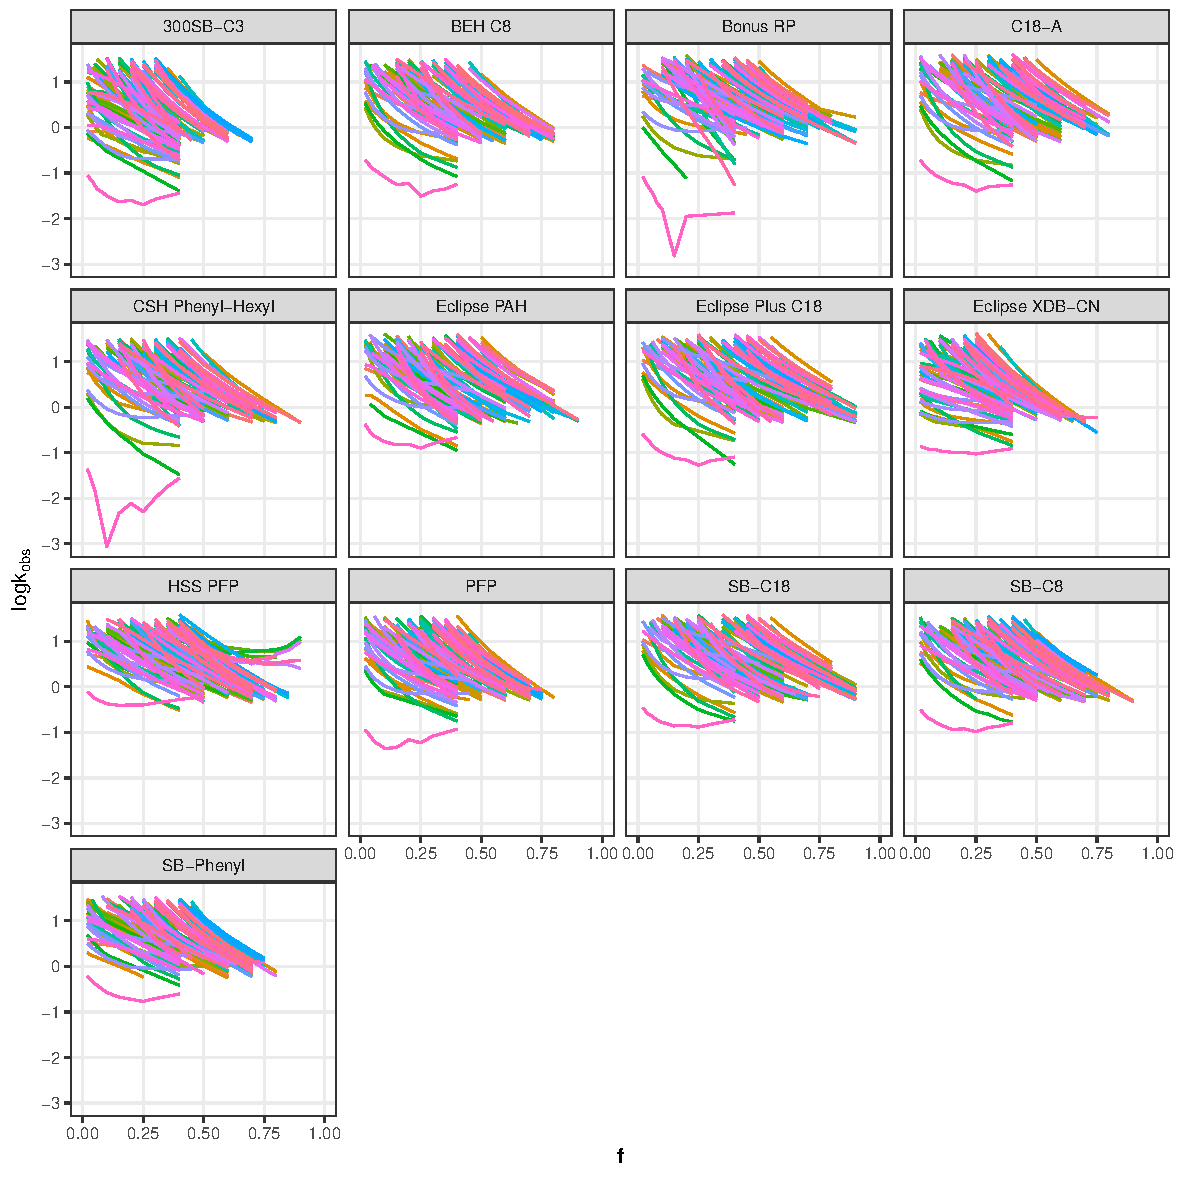
\includegraphics{../deliv/figures/manuscript/supplement/raw-data.pdf}

\newpage{}

\hypertarget{figure-s2.-utility-function.}{%
\section{Figure S2. Utility
function.}\label{figure-s2.-utility-function.}}

\[
\begin{aligned}
d &= \left| \log k_1 - \log k_2 \right|, \\
l_o &= 10^{\min\left(\log k_1,\ \log k_2\right)}, \\
h_i &= 10^{\max\left(\log k_1,\ \log k_2\right)}, \\
U &=
\frac{1}{1 + e^{-(d - 0.07918125)/0.015}}
\times
\frac{1}{1 + e^{-(l_o - 2)/0.25}}
\times
\frac{1}{1 + e^{-(10 - h_i)/1.5}}.
\end{aligned}
\]

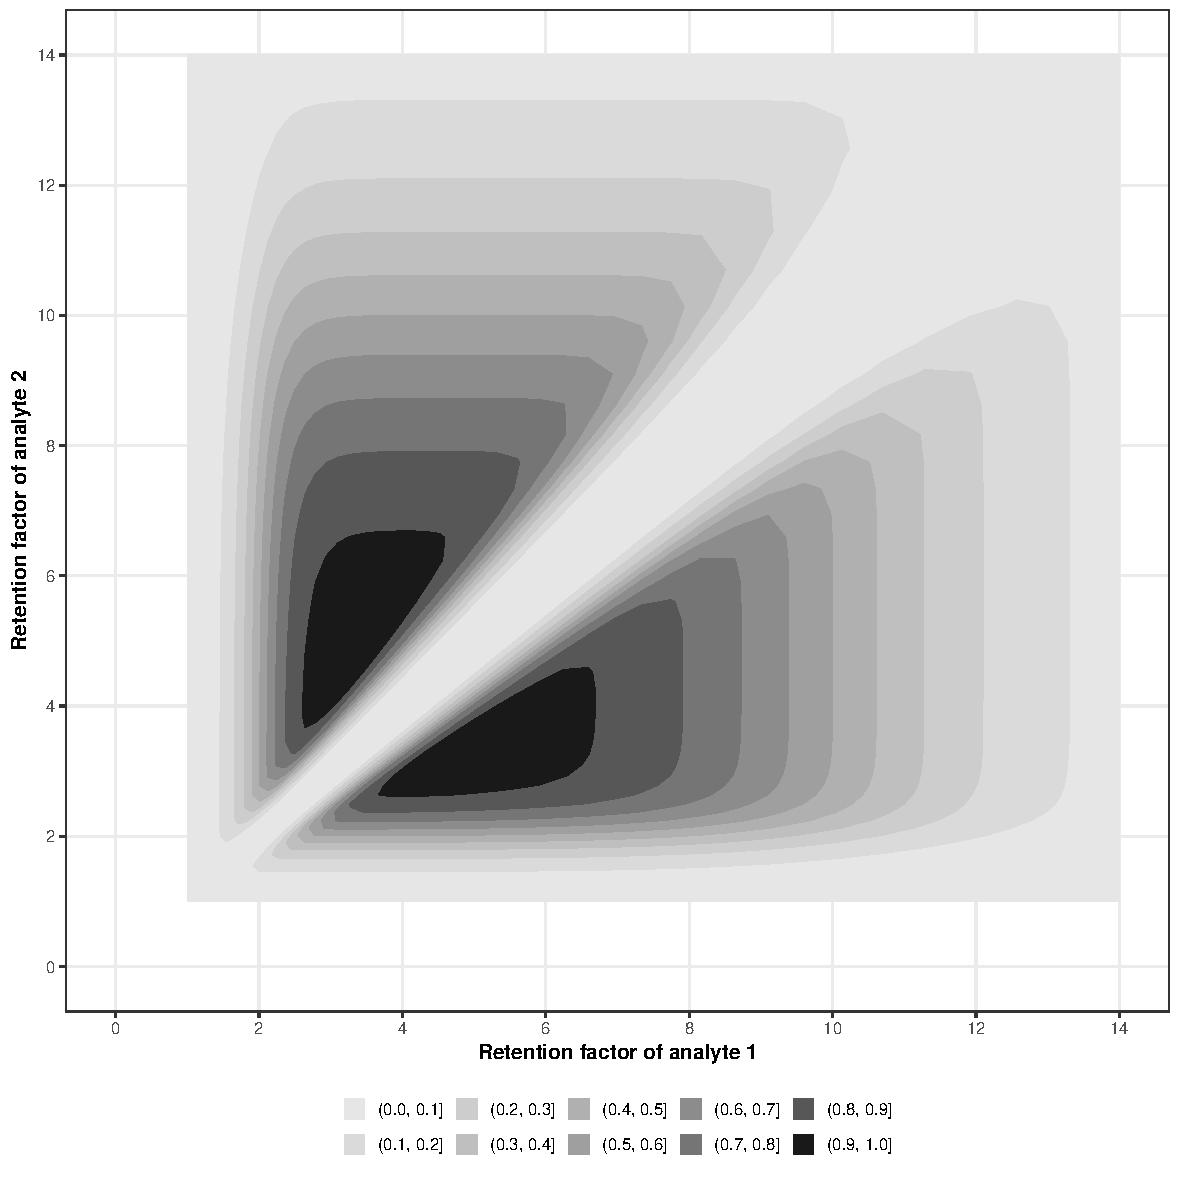
\includegraphics{../deliv/figures/manuscript/supplement/utylity-1.pdf}

\newpage{}

\hypertarget{figure-s3.-residuals}{%
\section{Figure S3. Residuals}\label{figure-s3.-residuals}}

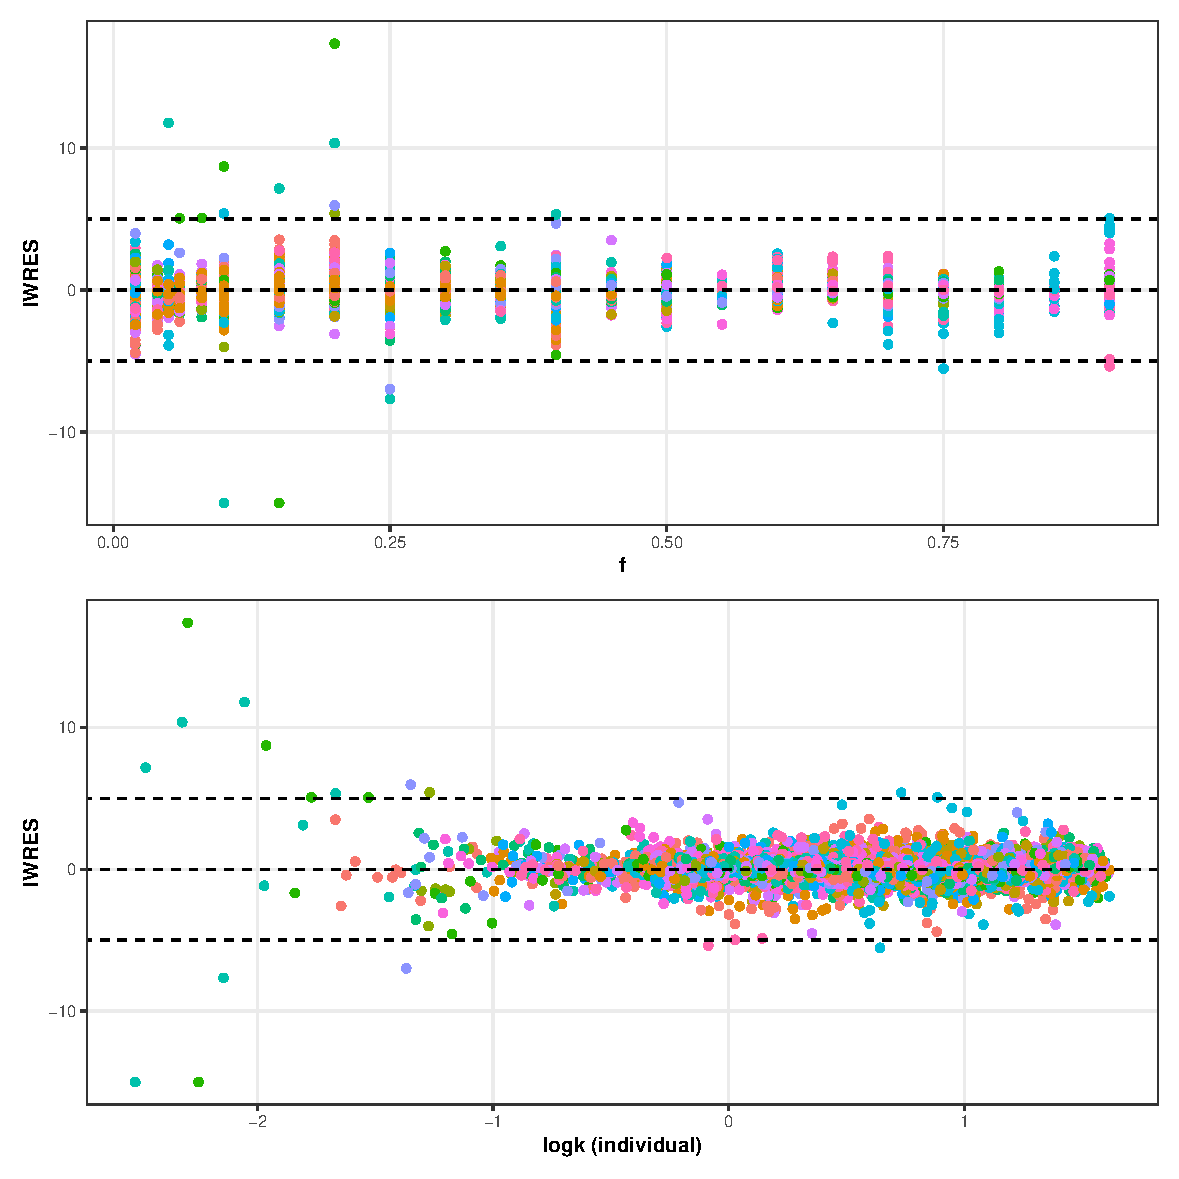
\includegraphics{../deliv/figures/manuscript/supplement/residuals.pdf}

\newpage{}

\hypertarget{figure-s4.-gof-plots-for-6-analytes}{%
\section{Figure S4. GOF plots for 6
analytes}\label{figure-s4.-gof-plots-for-6-analytes}}

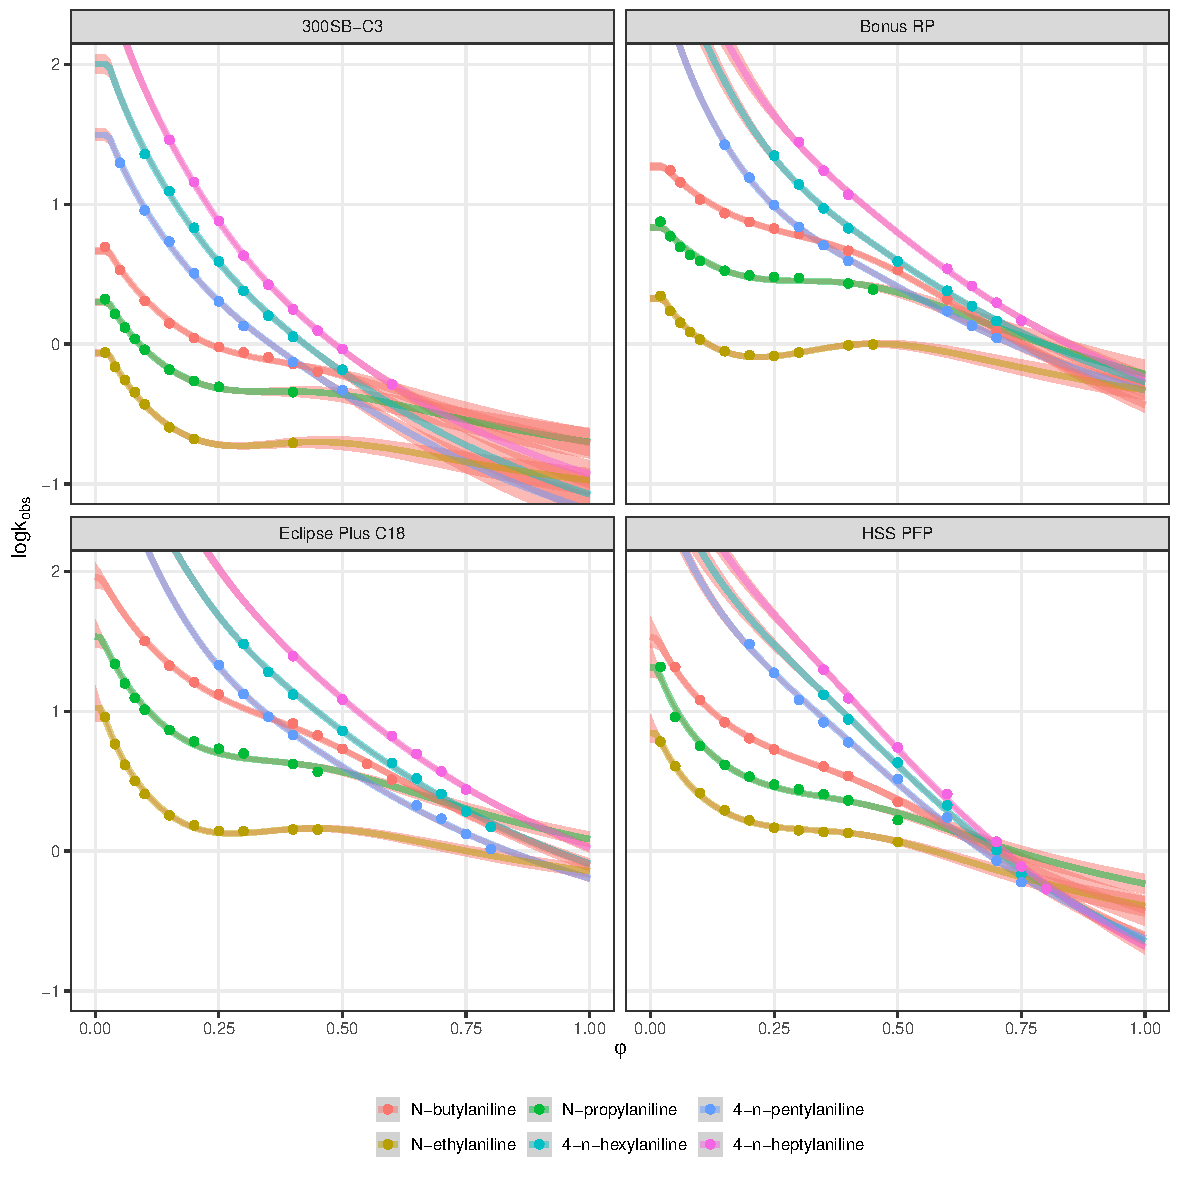
\includegraphics{../deliv/figures/manuscript/supplement/analyte-fits-example.pdf}

\newpage{}

\hypertarget{figure-s5.-etas}{%
\section{Figure S5. Etas}\label{figure-s5.-etas}}

eta\textsubscript{a} represents the deviation of an individual analyte's
parameter from its expected population-level value for a typical column,
assuming no interactions.

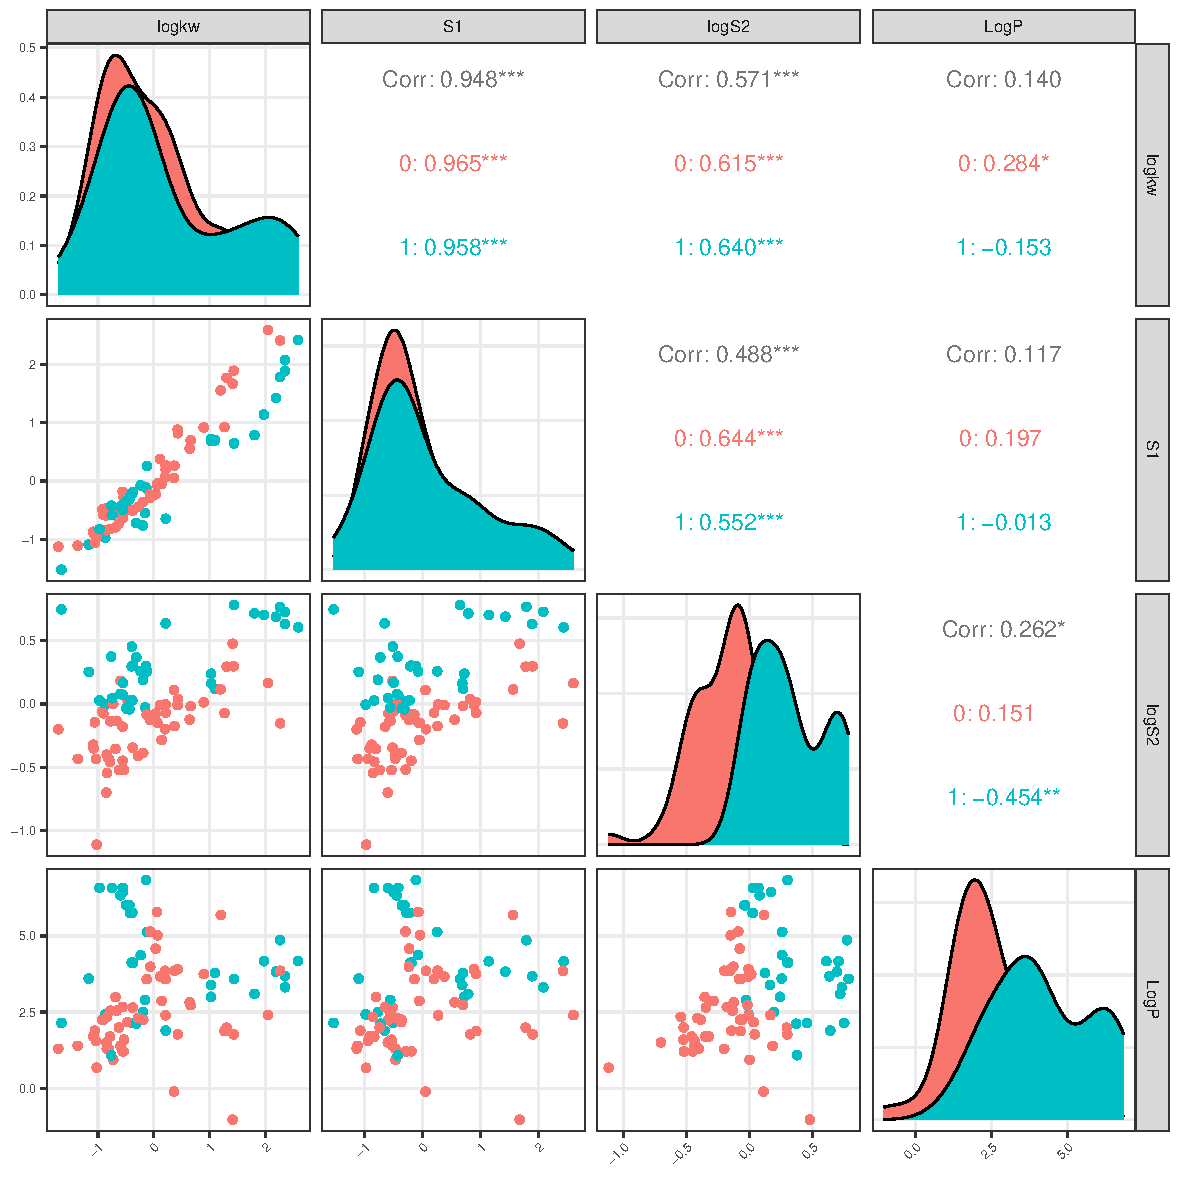
\includegraphics{../deliv/figures/manuscript/supplement/etas.pdf}

\newpage{}

\hypertarget{figure-s6.-kappas}{%
\section{Figure S6. Kappas}\label{figure-s6.-kappas}}

kappa\textsubscript{c} represents the deviation of an individual
analyte's parameter from its expected population-level value for a
typical analyte, assuming no interactions. The numbers correspond to
specific columns (stationary phases). The legend is provided in Table
2S.

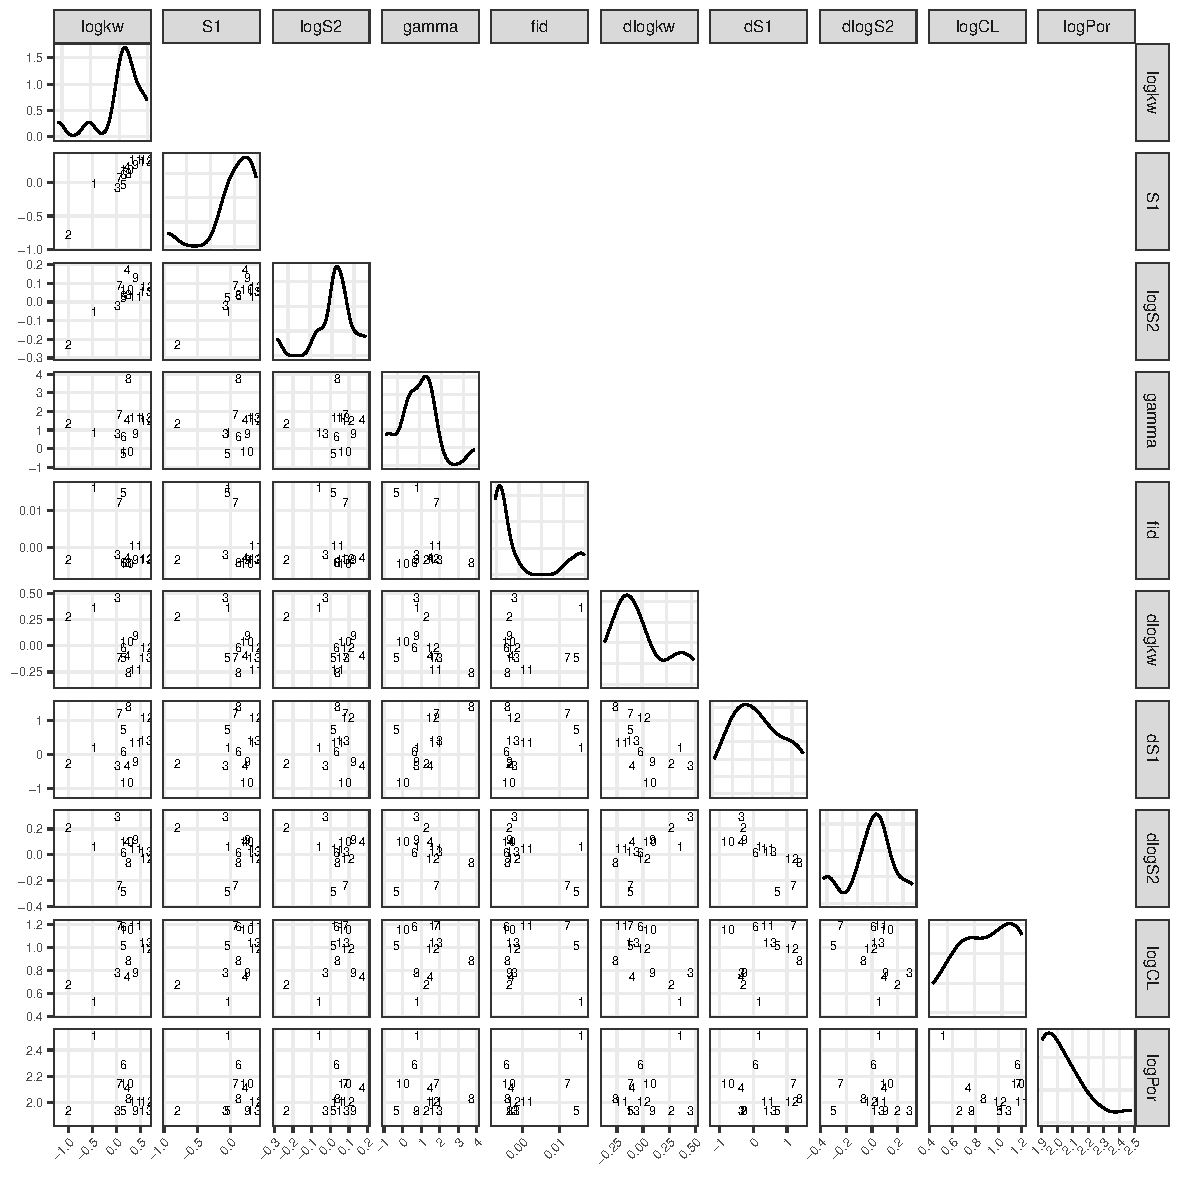
\includegraphics{../deliv/figures/manuscript/supplement/kappas-1.pdf}

\newpage{}

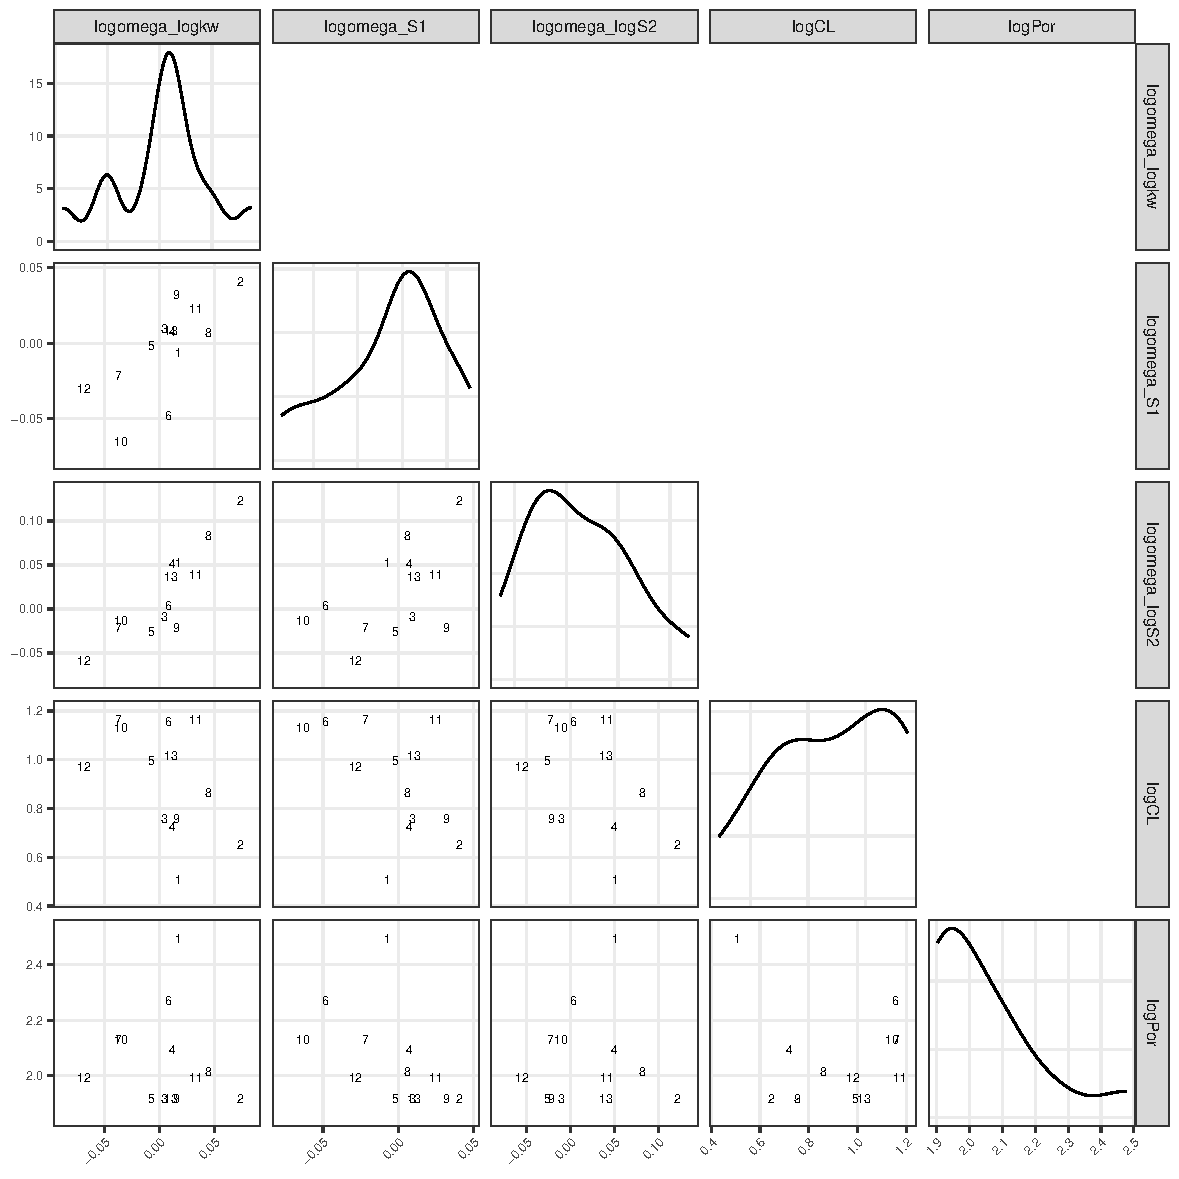
\includegraphics{../deliv/figures/manuscript/supplement/kappas-2.pdf}

\newpage{}

\hypertarget{figure-s7.-dzetas}{%
\section{Figure S7. Dzetas}\label{figure-s7.-dzetas}}

dzeta\textsubscript{a,c} represents analyte-column interactions.

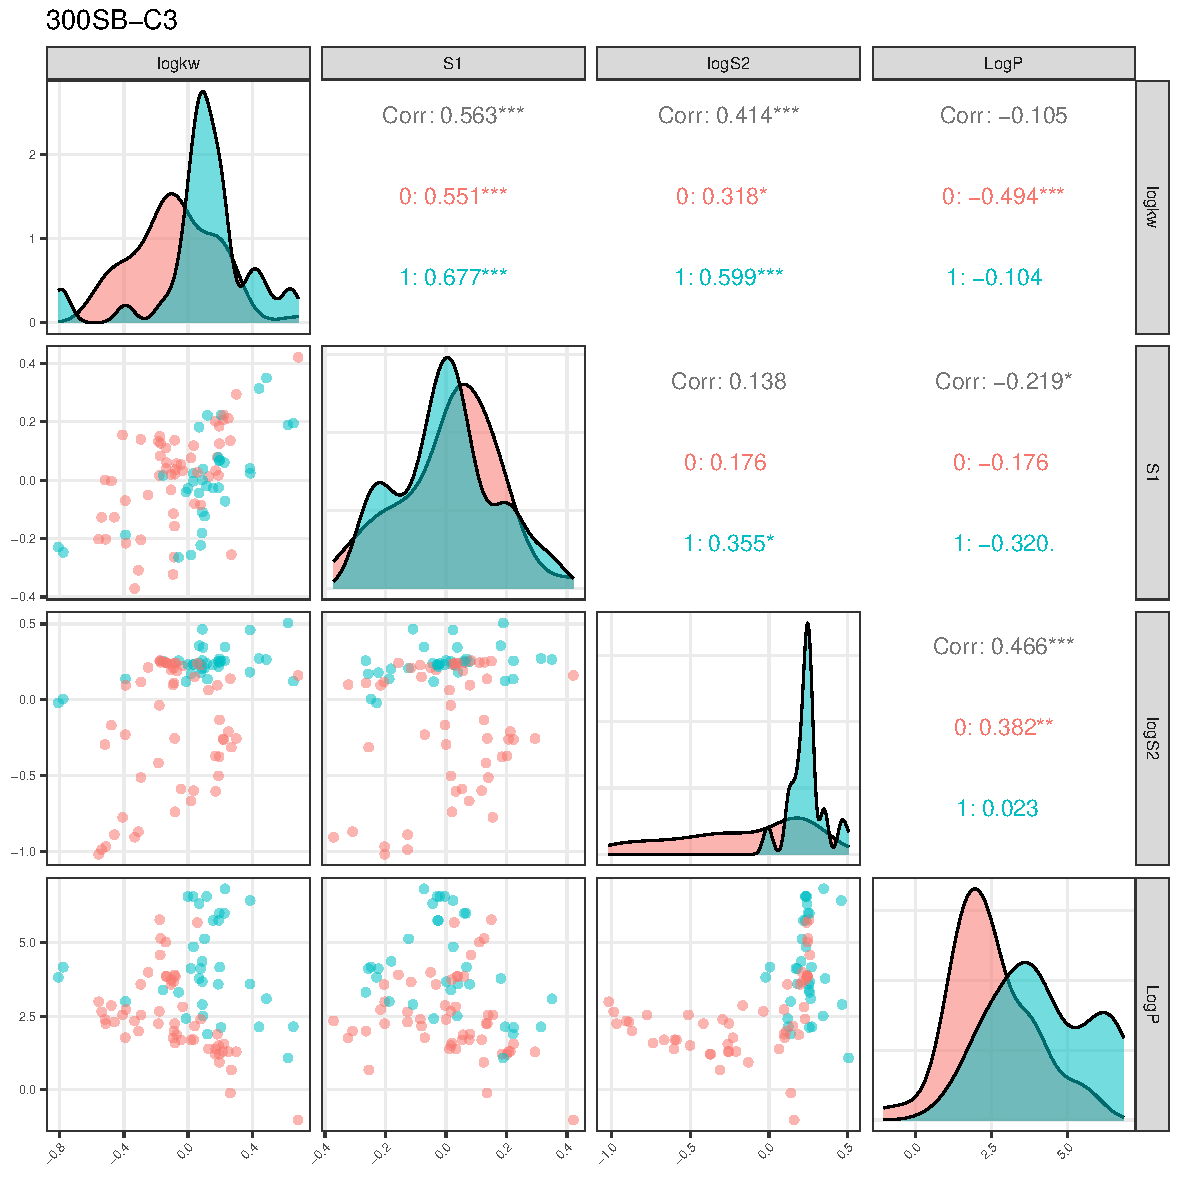
\includegraphics{../deliv/figures/manuscript/supplement/dzeta-1.pdf}

\newpage{}

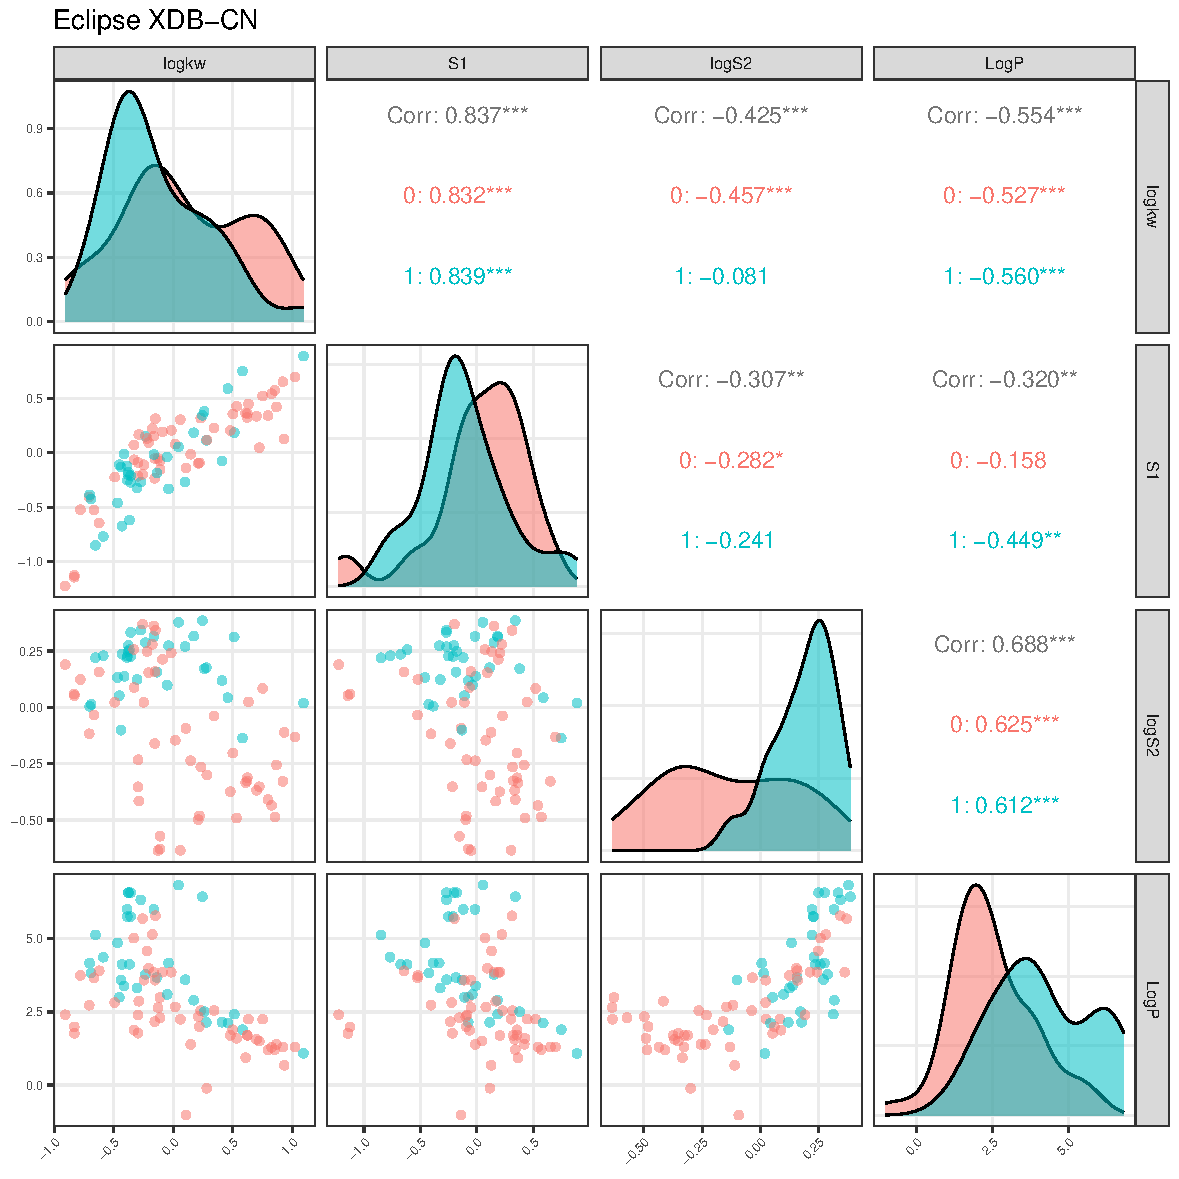
\includegraphics{../deliv/figures/manuscript/supplement/dzeta-2.pdf}

\newpage{}

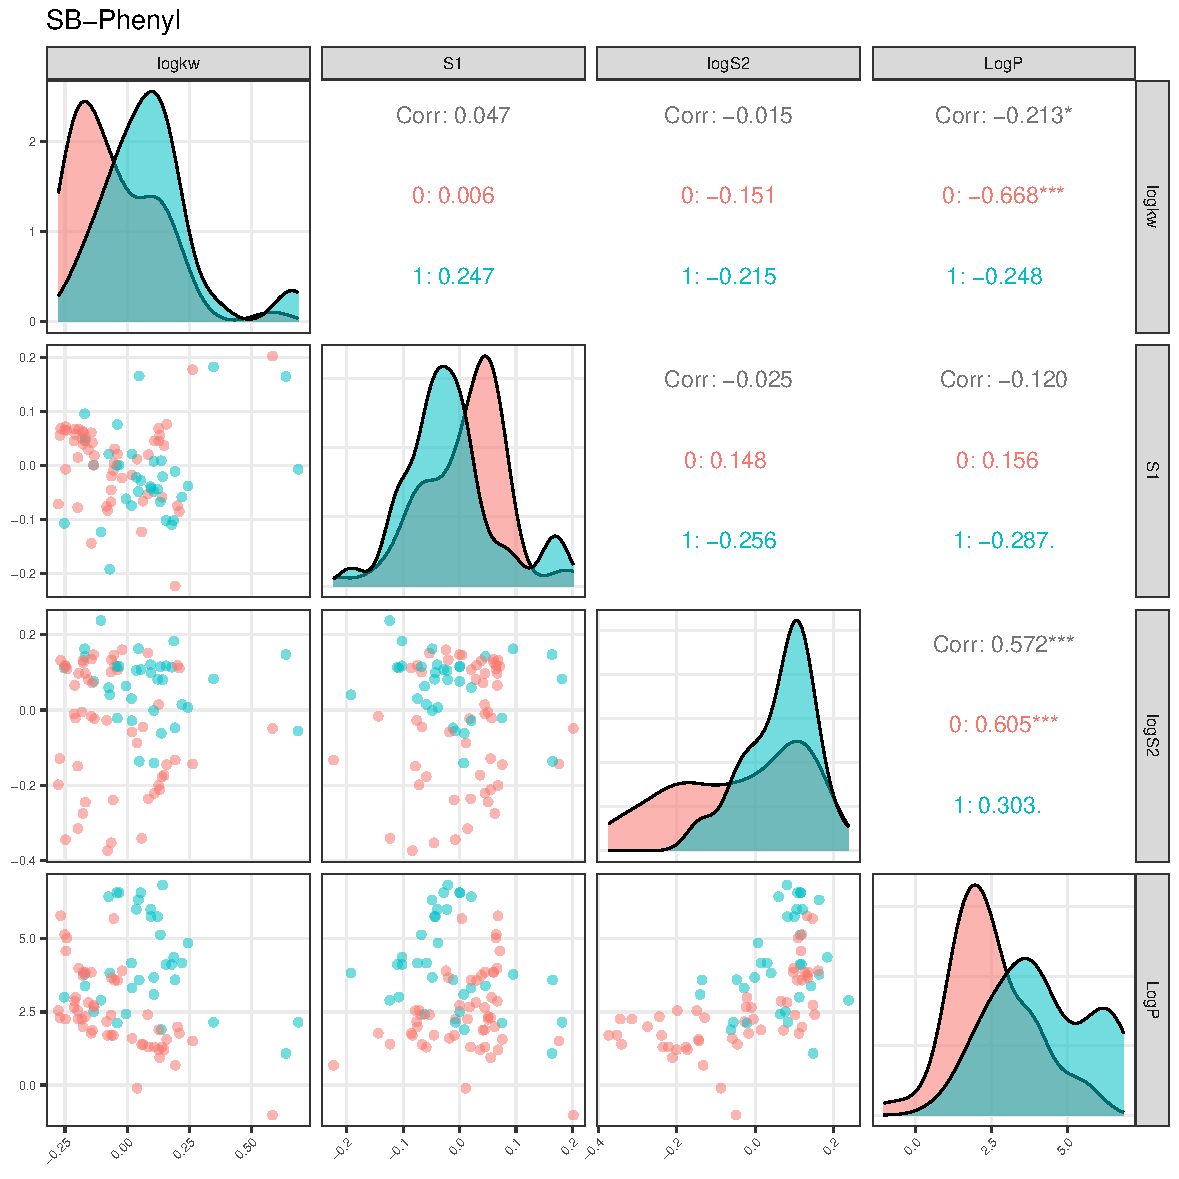
\includegraphics{../deliv/figures/manuscript/supplement/dzeta-3.pdf}

\newpage{}

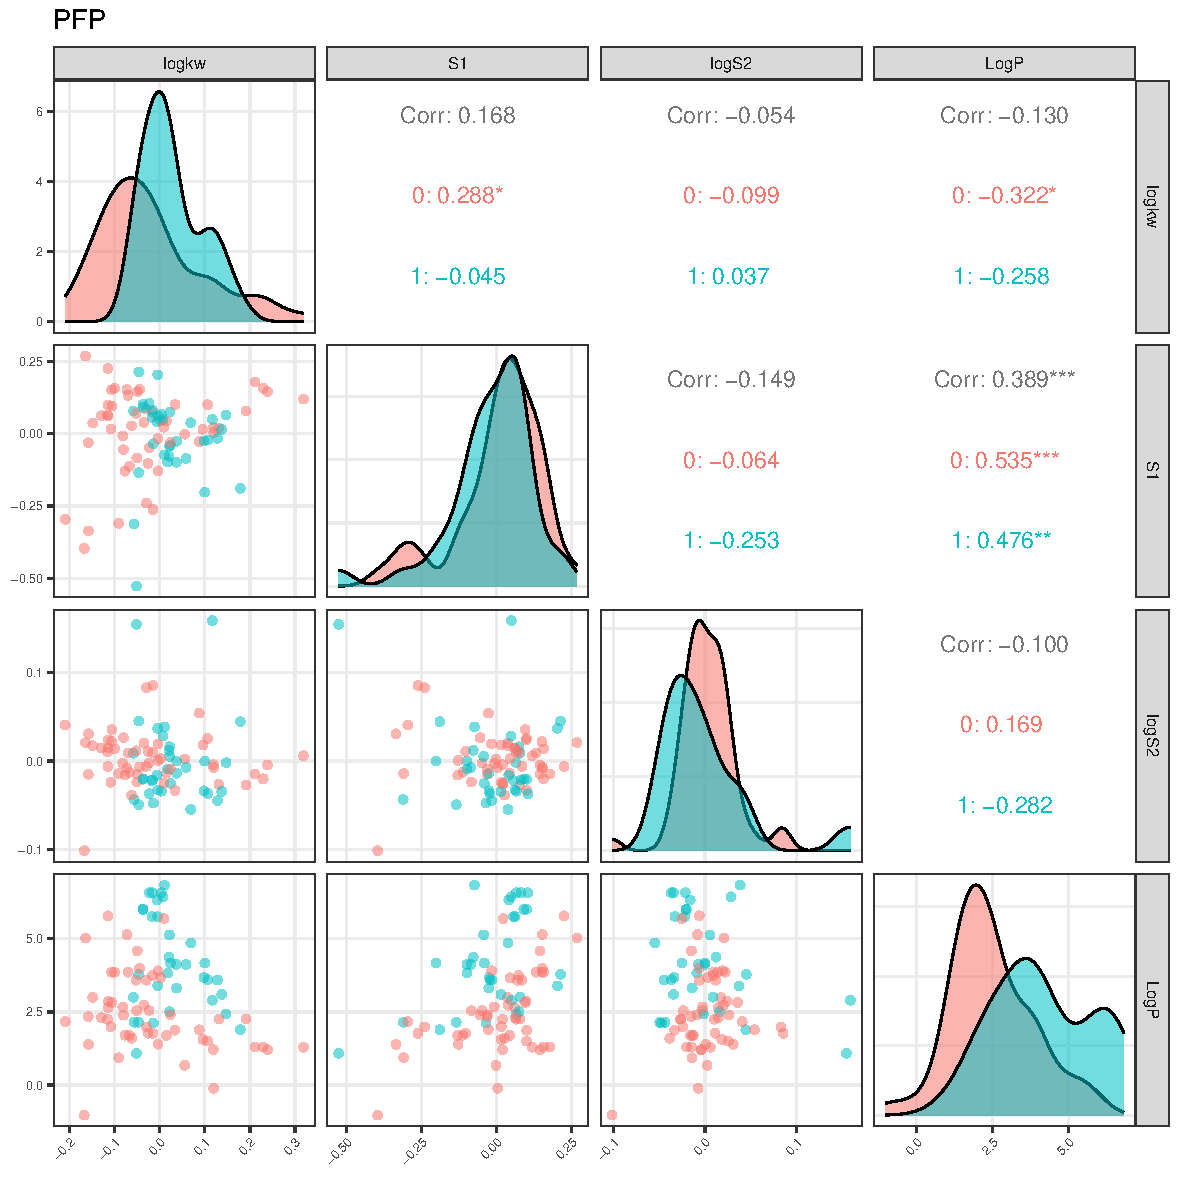
\includegraphics{../deliv/figures/manuscript/supplement/dzeta-4.pdf}

\newpage{}

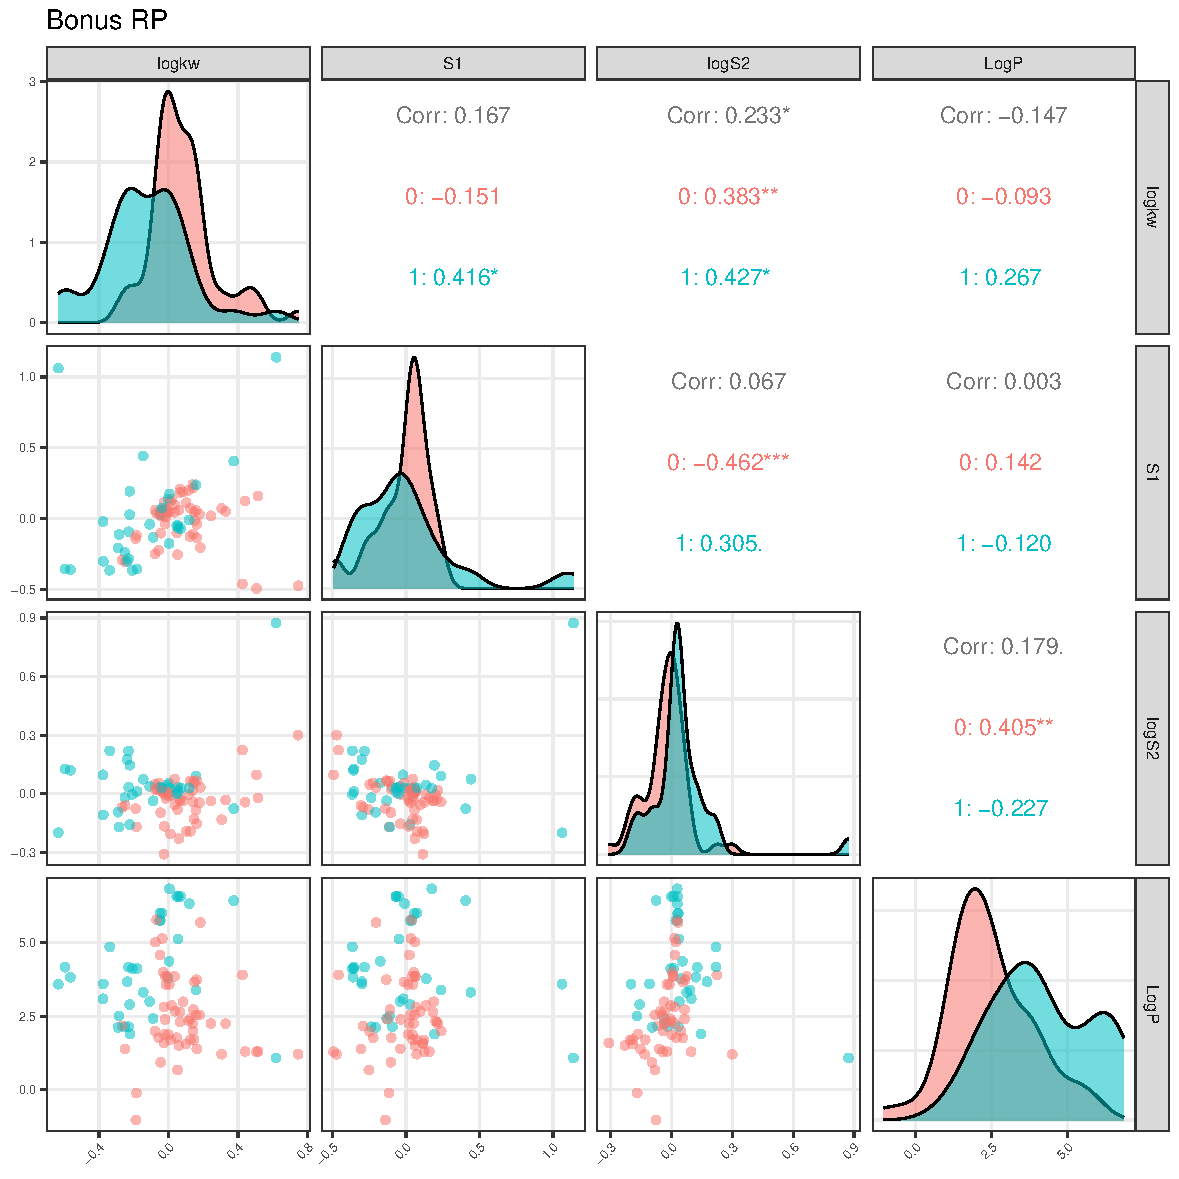
\includegraphics{../deliv/figures/manuscript/supplement/dzeta-5.pdf}

\newpage{}

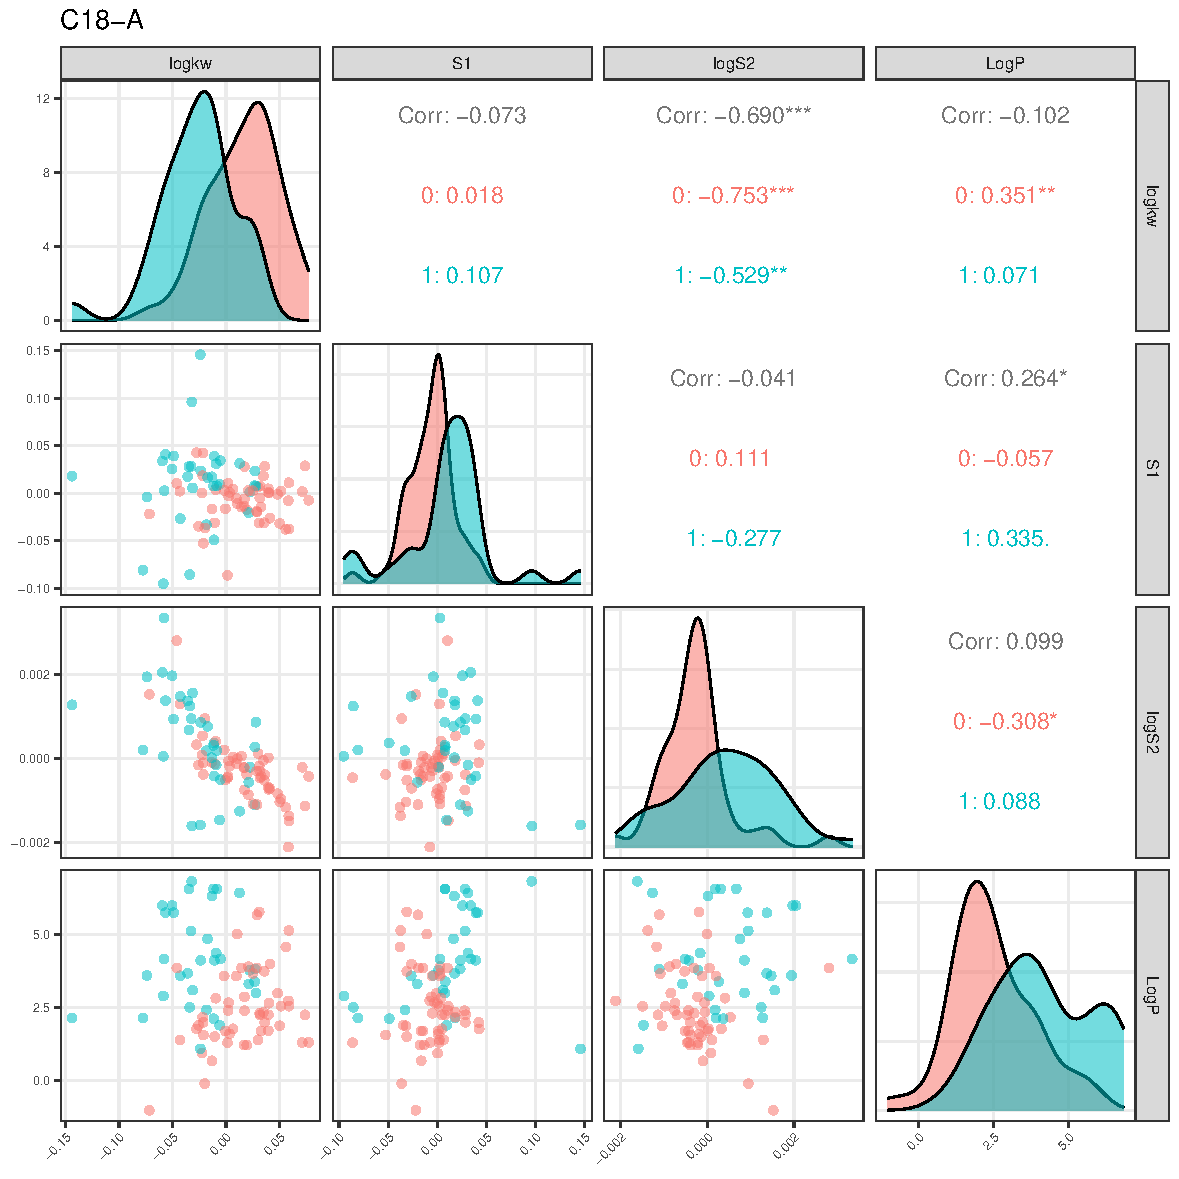
\includegraphics{../deliv/figures/manuscript/supplement/dzeta-6.pdf}

\newpage{}

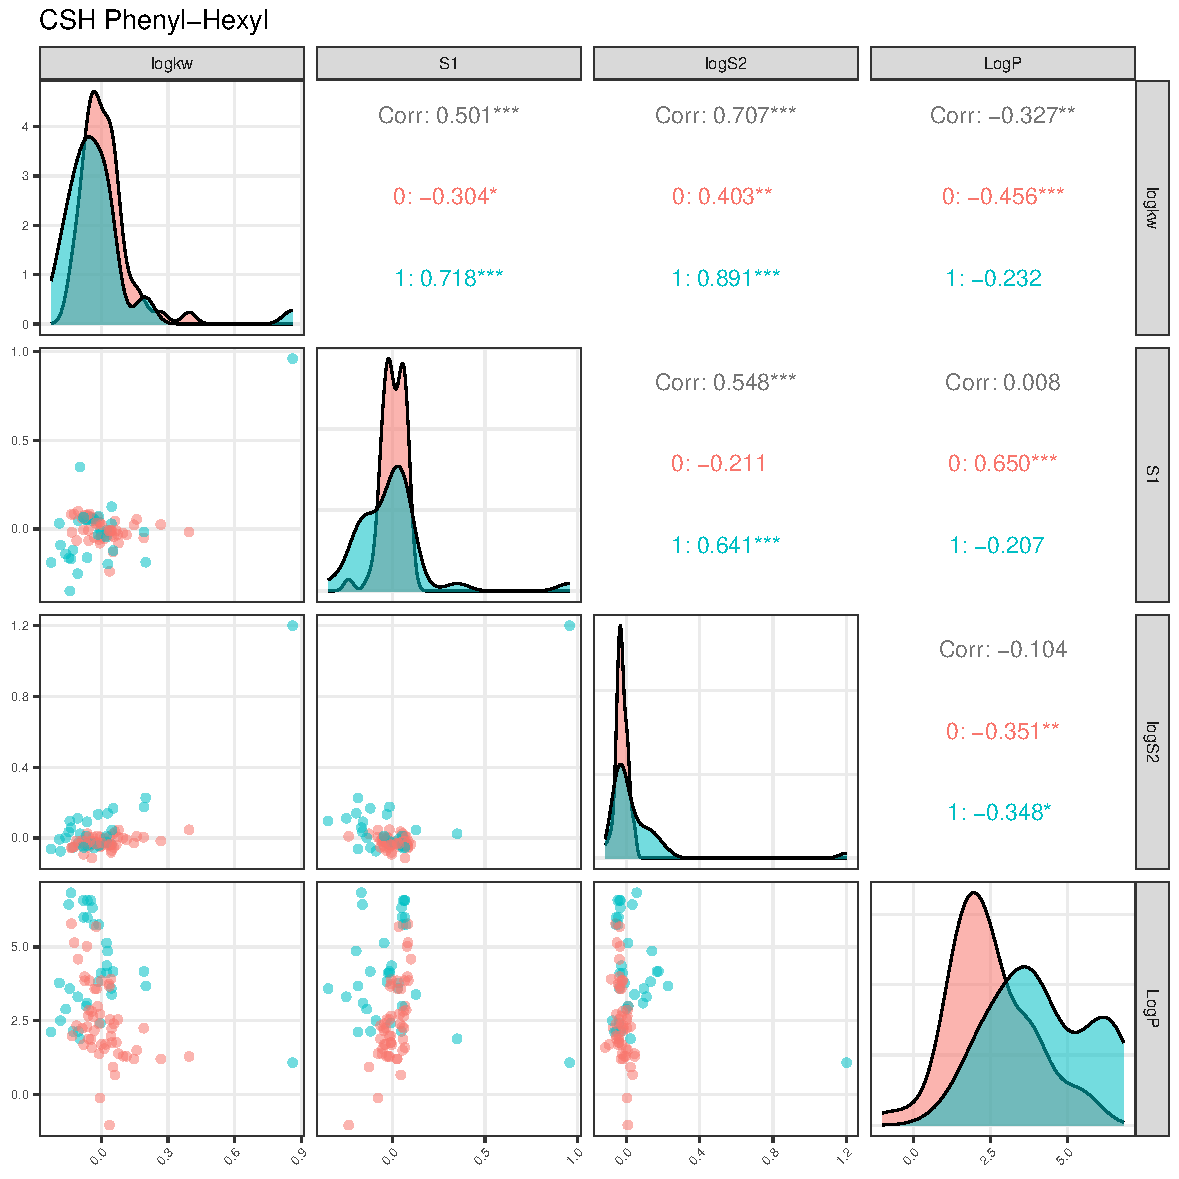
\includegraphics{../deliv/figures/manuscript/supplement/dzeta-7.pdf}

\newpage{}

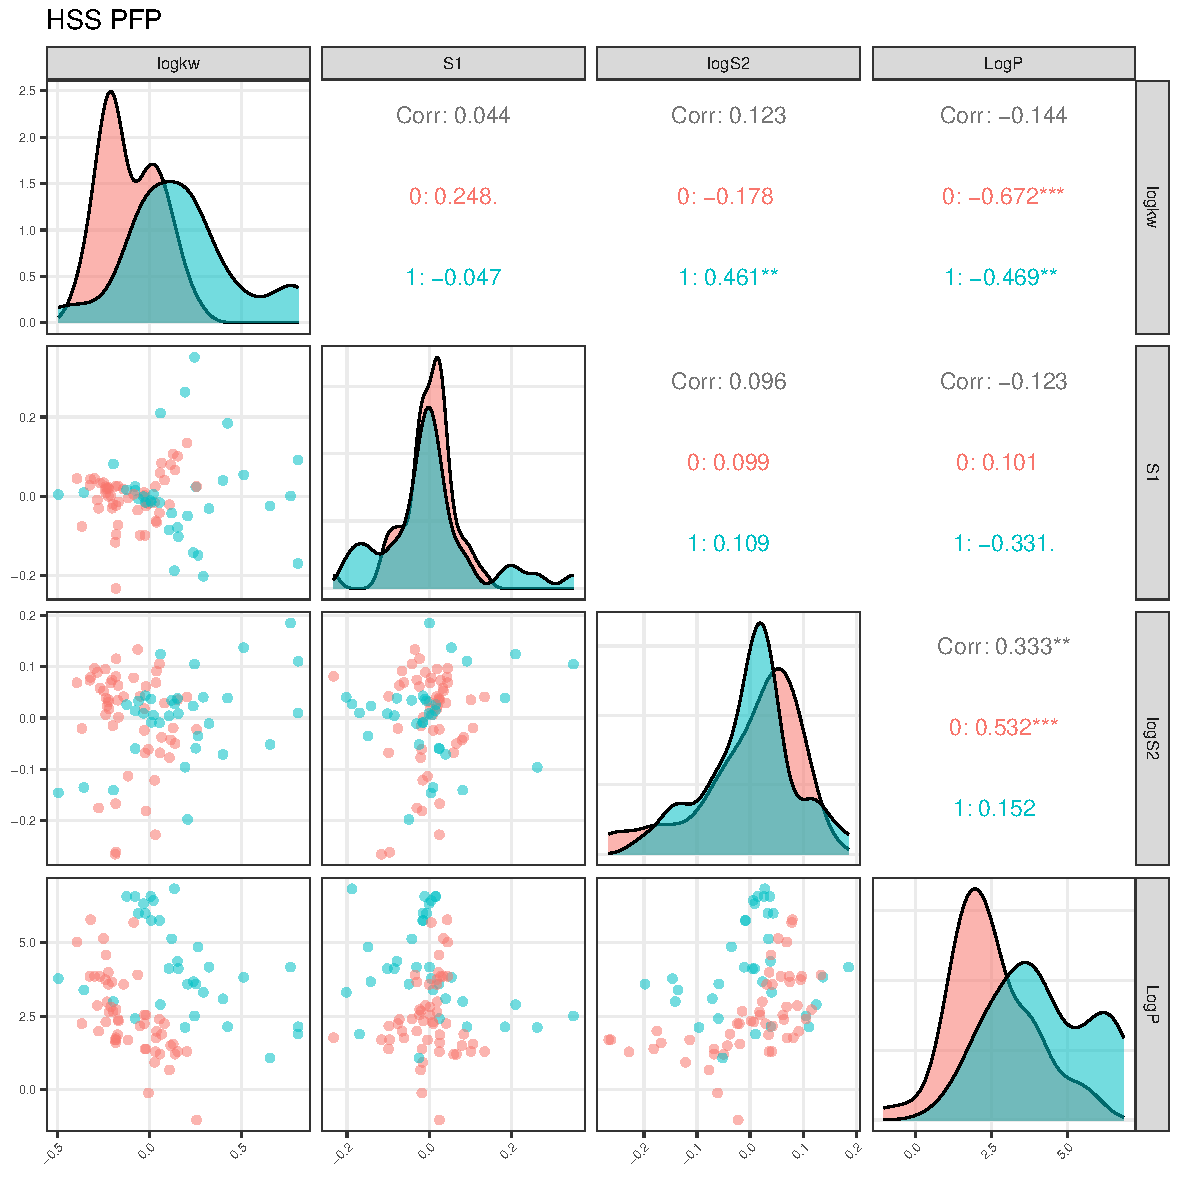
\includegraphics{../deliv/figures/manuscript/supplement/dzeta-8.pdf}

\newpage{}

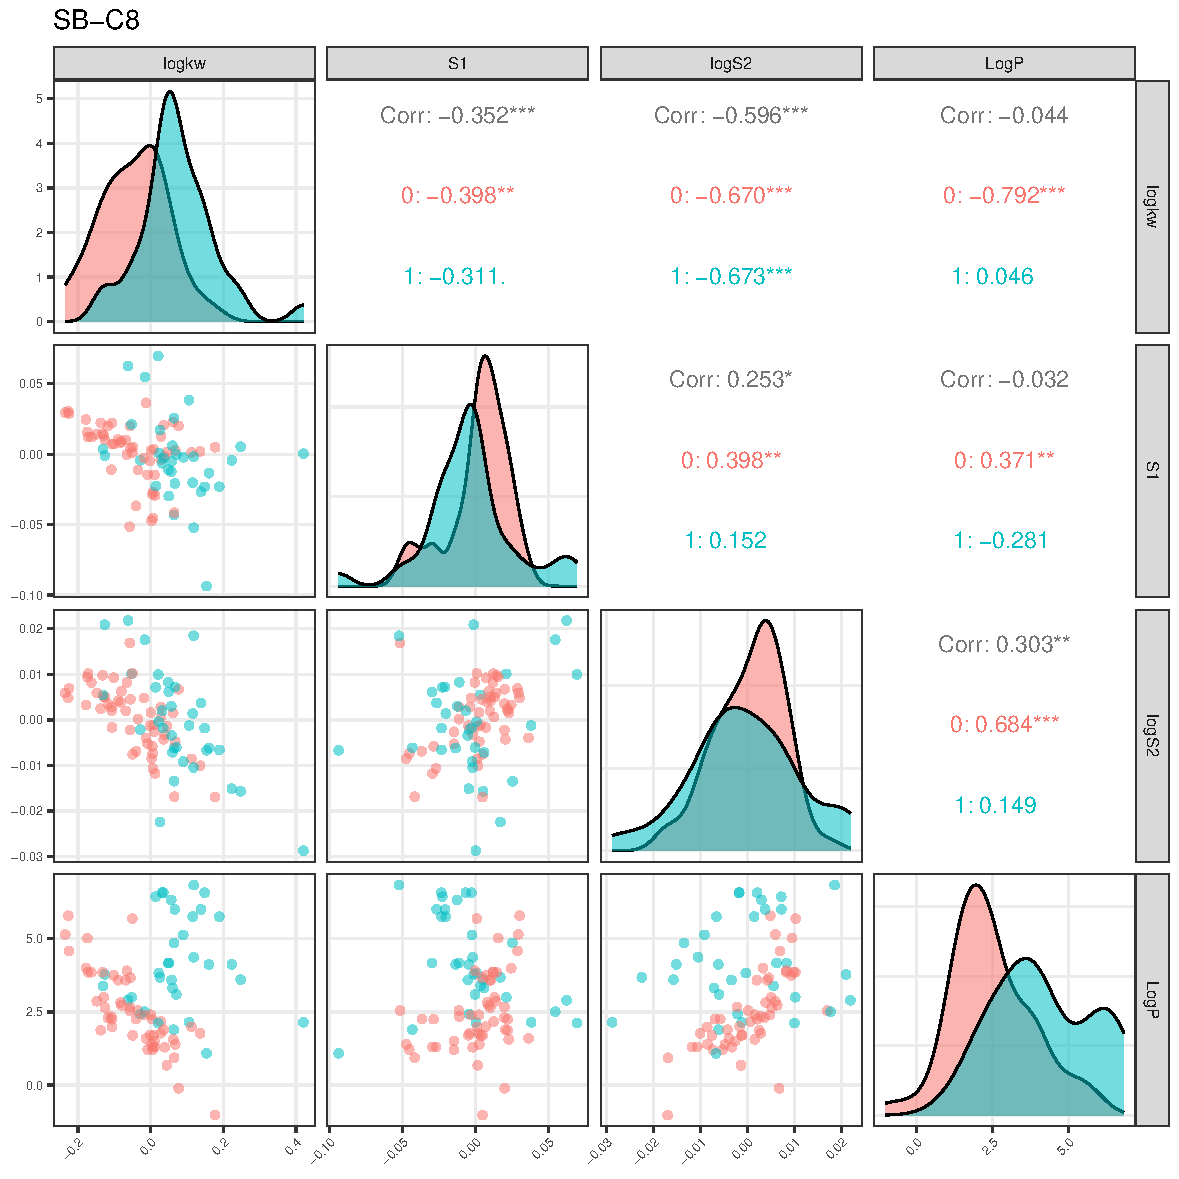
\includegraphics{../deliv/figures/manuscript/supplement/dzeta-9.pdf}

\newpage{}

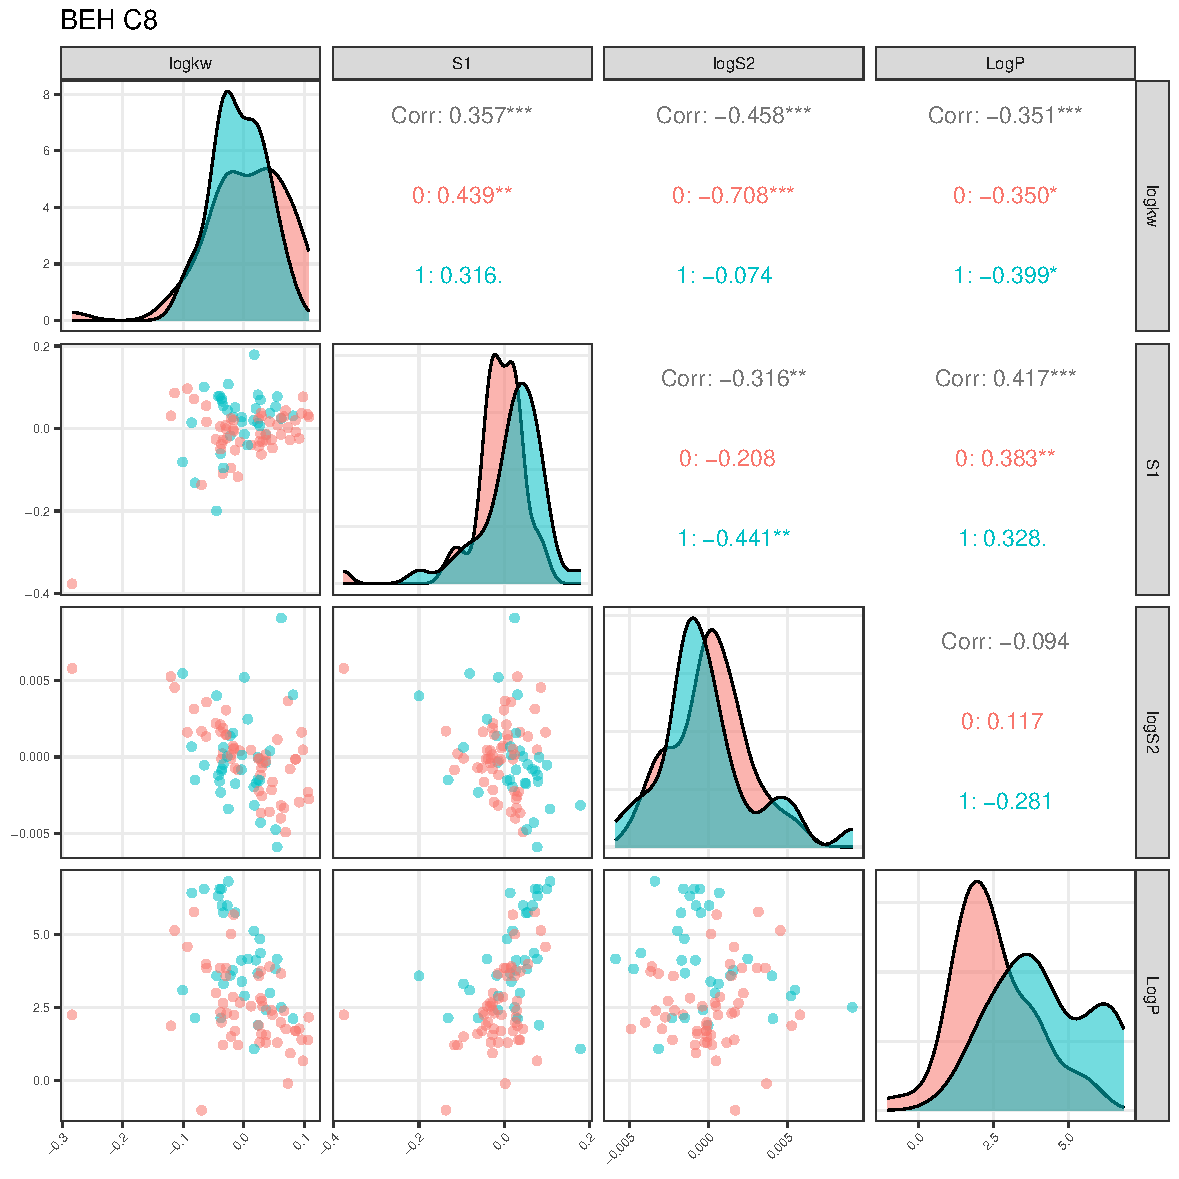
\includegraphics{../deliv/figures/manuscript/supplement/dzeta-10.pdf}

\newpage{}

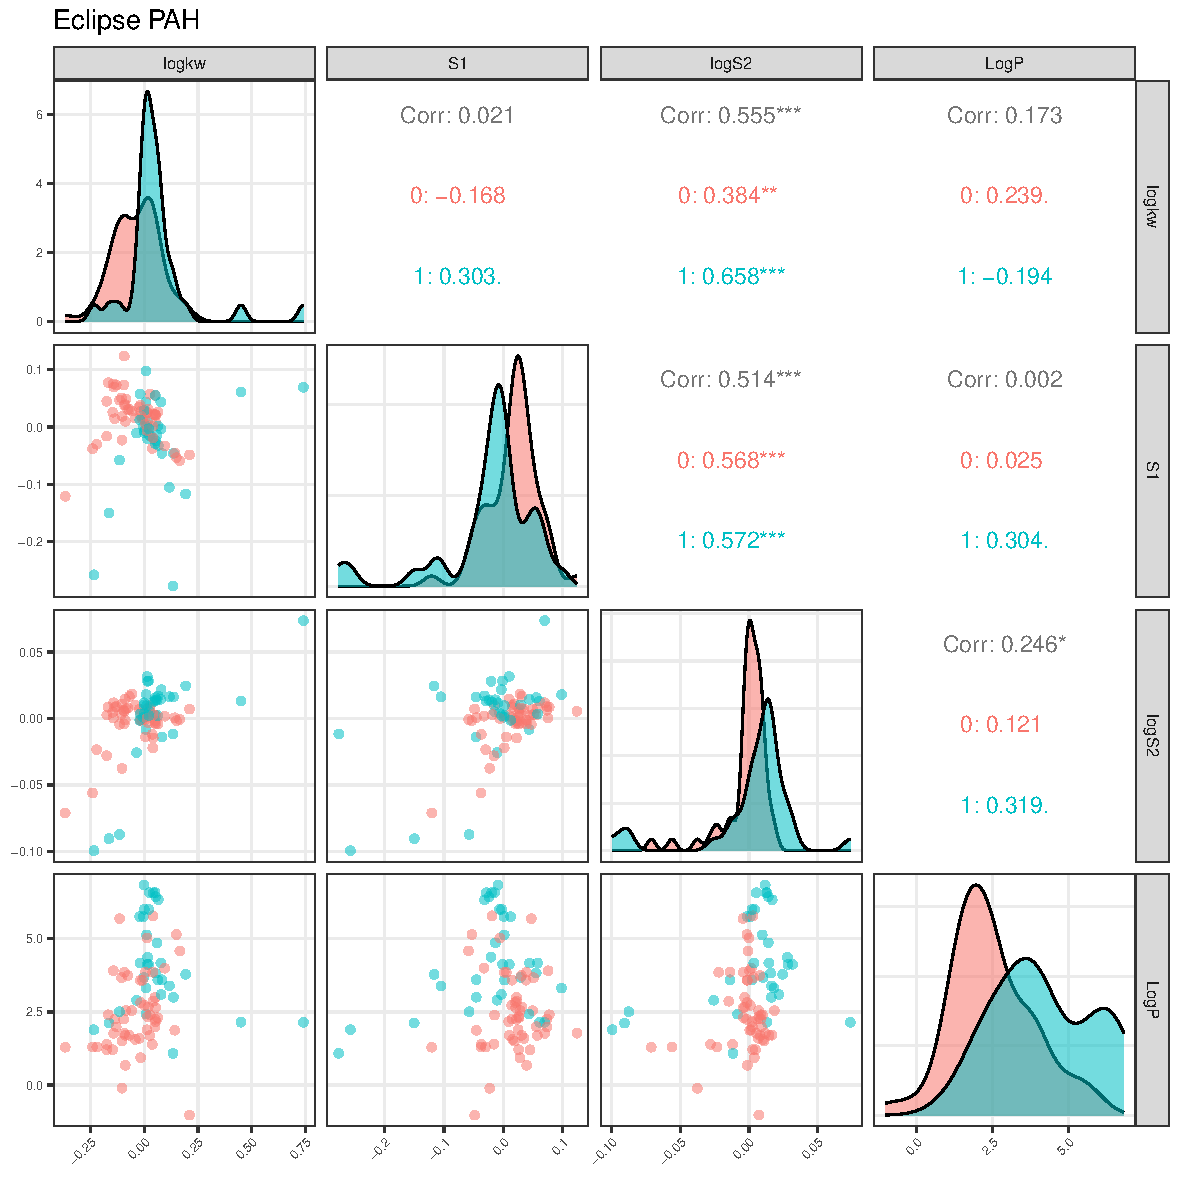
\includegraphics{../deliv/figures/manuscript/supplement/dzeta-11.pdf}

\newpage{}

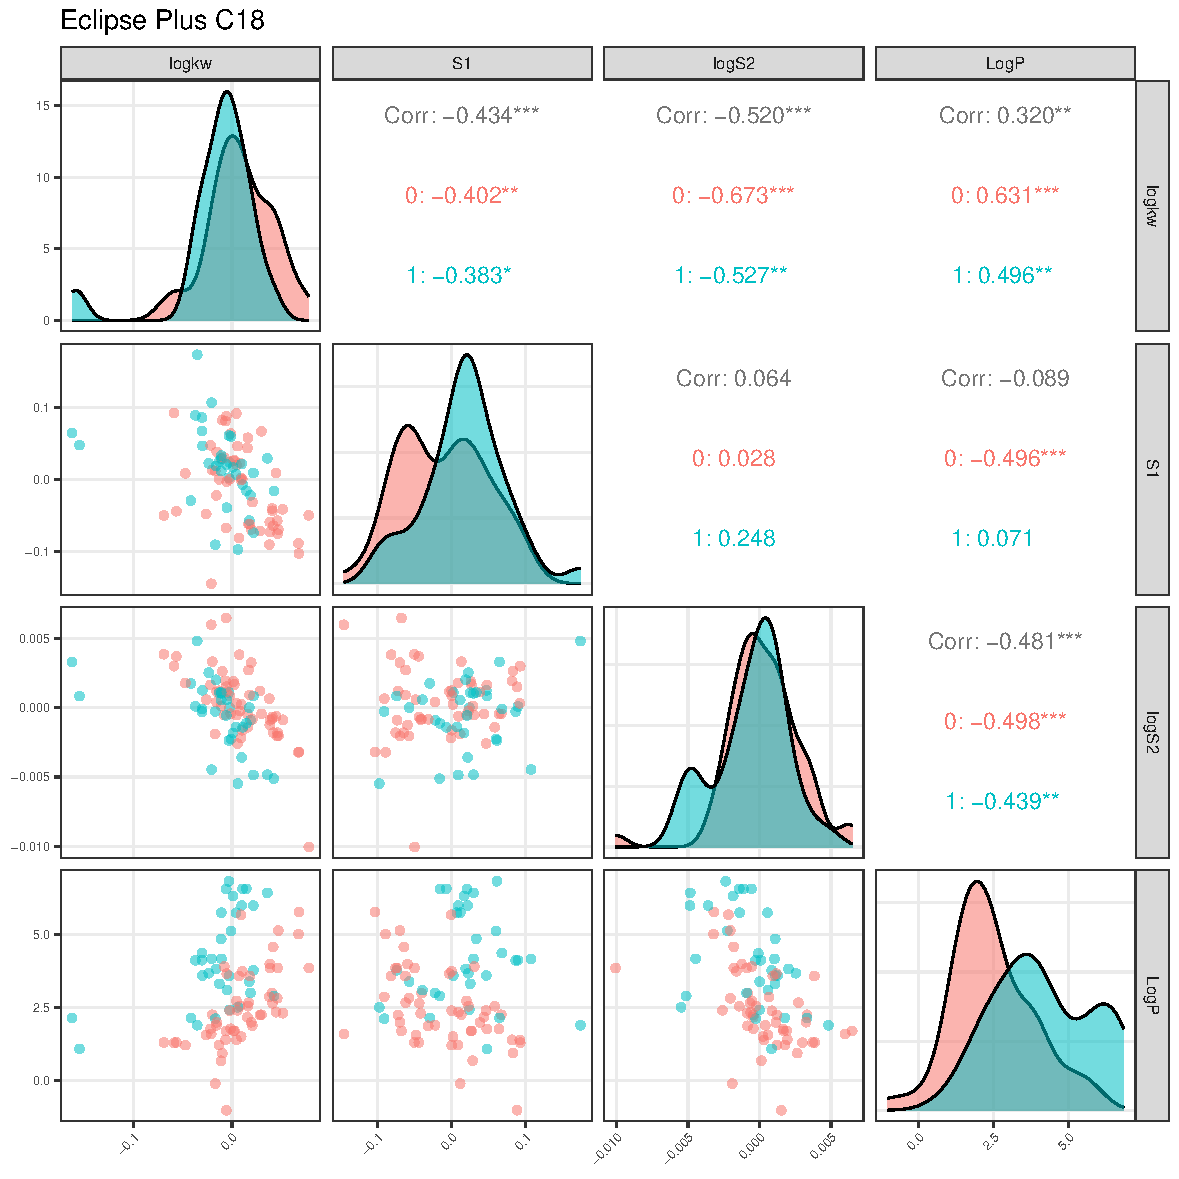
\includegraphics{../deliv/figures/manuscript/supplement/dzeta-12.pdf}

\newpage{}

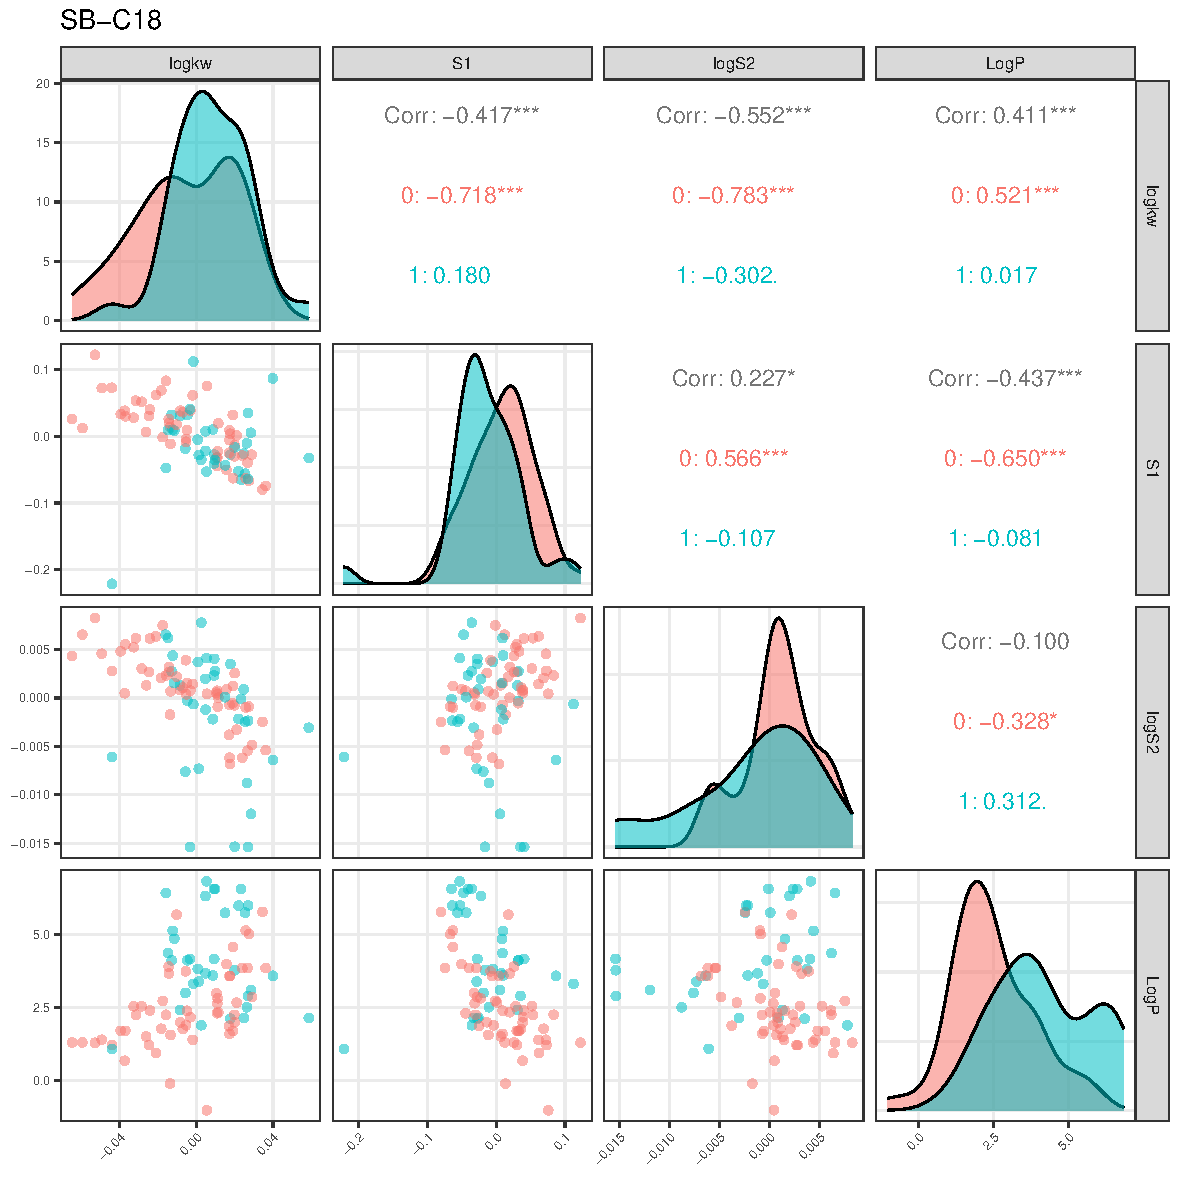
\includegraphics{../deliv/figures/manuscript/supplement/dzeta-13.pdf}

\newpage{}

\hypertarget{licenses}{%
\section*{Licenses}\label{licenses}}
\addcontentsline{toc}{section}{Licenses}

\begin{itemize}
\tightlist
\item
  Code \& copy; 2023, Paweł Wiczling, licensed under BSD-3.
\item
  Text \& copy; 2023, Paweł Wiczling, licensed under CC-BY-NC 4.0.
\end{itemize}

\hypertarget{original-computing-environment}{%
\section*{Original Computing
Environment}\label{original-computing-environment}}
\addcontentsline{toc}{section}{Original Computing Environment}

\begin{verbatim}
R version 4.3.1 (2023-06-16 ucrt)
Platform: x86_64-w64-mingw32/x64 (64-bit)
Running under: Windows 10 x64 (build 19045)

Matrix products: default


locale:
[1] LC_COLLATE=Polish_Poland.utf8  LC_CTYPE=Polish_Poland.utf8   
[3] LC_MONETARY=Polish_Poland.utf8 LC_NUMERIC=C                  
[5] LC_TIME=Polish_Poland.utf8    

time zone: Europe/Warsaw
tzcode source: internal

attached base packages:
[1] stats     graphics  grDevices utils     datasets  methods   base     

other attached packages:
[1] kableExtra_1.4.0 dplyr_1.1.4     

loaded via a namespace (and not attached):
 [1] vctrs_0.6.5       svglite_2.1.3     cli_3.6.2         knitr_1.46       
 [5] rlang_1.1.3       xfun_0.54         stringi_1.8.4     generics_0.1.3   
 [9] textshaping_0.4.0 jsonlite_1.8.8    glue_1.7.0        colorspace_2.1-0 
[13] htmltools_0.5.8.1 ragg_1.3.2        scales_1.3.0      fansi_1.0.6      
[17] rmarkdown_2.27    munsell_0.5.1     evaluate_1.0.3    tibble_3.2.1     
[21] fastmap_1.2.0     yaml_2.3.8        lifecycle_1.0.4   stringr_1.5.1    
[25] compiler_4.3.1    codetools_0.2-19  pkgconfig_2.0.3   rstudioapi_0.16.0
[29] systemfonts_1.1.0 digest_0.6.35     viridisLite_0.4.2 R6_2.5.1         
[33] tidyselect_1.2.1  utf8_1.2.4        pillar_1.9.0      magrittr_2.0.3   
[37] withr_3.0.2       tools_4.3.1       xml2_1.3.6       
\end{verbatim}



\end{document}
